
\section{Evaluation}
\label{sec:Evaluation}
We first described the simulation setup, then present the simulation results.

\subsection{Simulation setup}

\subsubsection{Experimental Parameter}
For any VN request, the number of VN nodes is randomly determined by a uniform distribution between $\VirtualNodeSizeMinimum$ and $\VirtualNodeSizeMaximum$ and each pair of virtual nodes is randomly connected with probability of $\VirtualNodenodeProbability$, and ensure the VN is connected graph. The computing demand on VN nodes follow a uniform distribution from $\VirtualNodeComputationMinimum$ to $\VirtualNodeComputationMaximum$, as well as the bandwidth on VN links from $\VirtualEdgeBandwithMinimum$ to $\VirtualEdgeBandwithMaximum$.

%VN requests arrive randomly over a timespan of $\PhysicalNewtorkRunTimeInterval$ time slots and the inter-arrival time is
%assumed to follow the Geometric distribution at a rate of $\requestAppearProbability$ per time slot. The resource lease times of each VN request follows the uniform distribution as well at a rate  range from $\VNRequestsContinueTimeMinimum$ and $\VNRequestsContinueTimeMaximum$ per time slot.
The arrivals of VN requests are modeled by a Poisson process (with mean of \PossionMean \ requests per 1 time units).
The duration of the requests follows an exponential distribution with $\VNRequestsContinueTimeExponentialMean$ time units on average.
A high request rate and long lease time ensures that the physical infrastructure is operating at high utilization. we supposed a assumption that each virtual node of VN should be mapped on only one isolated  physical node.
%The arrivals of VN requests are modeled by a Poisson process (with mean of \PossionMean requests per 1 time units).
%The duration of the requests follows an exponential distribution with $\VNRequestsContinueTimeExponentialMean$ time units on average

We assumed the relative cost of computing demand  compared with bandwidth demand is $\RelativeCostbetweenComputingBandwidth$ according to  \cite{armbrust2009above,yu2010survivable}, which means $\lambda/\alpha=\RelativeCostbetweenComputingBandwidth$.
%The SN topologies used are randomly generated with $\SubStrateNodeSize$ nodes using the GT-ITM tool  \cite{zegura1996model}.
The SN topologies used from SNDlib topology data \cite{orlowski2010sndlib} as shown in Tab.\ref{tab:SNDlibTopo}.
The computing(bandwidth) resources of the physical nodes (links) are integer uniformly distributed between $\SubStrateNodeComputationMinimum$ and $\SubStrateNodeComputationMaximum$ ($\SubStrateEdgeBandwithMinimum$ and $\SubStrateEdgeBandwithMaximum$), respectively. To model the physical node failure scenario, we choose all nodes of physical network to fail one by one, and statistically calculating migration frequency in every $\SubStrateFacilityNodeFailDuration$ time units.
\begin{table}[htb]
\centering
\caption{SNDlib topology data}\label{tab:SNDlibTopo}
\begin{tabular}{|c|c|c|}
  \hline
  % after \\: \hline or \cline{col1-col2} \cline{col3-col4} ...
  name & node & edge \\
  \hline
  cost266& 37& 57\\
  geant& 22& 36\\
  germany50& 50& 88\\
  giul39& 39& 172\\
  janos-us-ca& 39& 122\\
  janos-us& 26& 84\\
  nobel-eu& 28& 41\\
  norway& 27& 51\\
  pioro40& 40& 89\\
  ta1& 24& 55\\
  ta2& 65& 108\\
  zib54& 54& 81\\
  \hline

\end{tabular}
\end{table}

%In our proposed star decomposition method for $\MyProblemAbrreviation$ problem, we employ a proactive failure dependent protection(FD) based $\MyProblemAbrreviation$ problem design with sufficient redundancy before embedding process in order to conquer the limitation of existing work, which consider the redundancy within the embedding process and failure independent protection based migration approach in resource efficiency.

For performance comparisons, besides our scheme (named by $\MyAlgorithmMethodAbrreviation$), we also implemented other survivable algorithms $\SecondAlgorithmMethodAbrreviation$ \cite{yeow2011designing} as follows:
\begin{itemize}
  \item $\SecondAlgorithmMethodAbrreviation$ : algorithm connect links between backup and critical nodes, between backup and backup nodes, but not connect links between critical and critical nodes. critical node denote the former physical node which is embedded with virtual nodes. backup node denote the added nodes.
  \item $\FouthAlgorithmMethodAbrreviation$: When every node of physical network mapped with virtual node fail, a simple method is that add a new  physical node for migrating the failure virtual node and connect new link with the failure link in terms of the failure physical node.
\end{itemize}

Moreover, All algorithm is  compared with a virtual network embedding algorithm\cite{liu2011completing} which is the embedding method when virtual network request firstly arrived, where VN do not have survivability requirement, and the virtual network embedding request (labeled $\ThirdAlgorithmMethodAbrreviation$) as a baseline to gauge the amount of added resources consumed for survivability, label "algorithm shared" or "algorithm Noshared" in experimental evaluation figures. We supposed that when a virtual network is embedded in physical network, the successful survivable guarantee has been supposed  with respect to algorithm $\ThirdAlgorithmMethodAbrreviation$.

Based on the resource of physical network whether shared or non-shared(dedicated) \cite{lu2006efficient}, we independently implement the two situation with respect to resource distribution pattern. The physical resource corresponding augment backup demand of  every virtual network request with survivable guarantee  could be shared with each other. Dedicated means that for each virtual network a
complete backup network can be set up and backup resources are fully dedicated to the virtual networks and independent from each other. However, this is resource inefficient, since for each virtual resource that gets embedded a dedicated physical entity is needed. In some cases it might also be acceptable to share and reuse the backup resources in order to reduce the footprint on the physical network caused by the additional
backup resources. Usually, a higher degree of reused backup resources results in lower reliability, and vice versa.

Every virtual network's request exist a life lease time span, statistically record virtual or physical network's performance metric in real-time situation. Because the experimental data of every algorithm's performance metric fluctuate, we incrementally record experimental data of every virtual or physical network performance metric, then average the experimental data by successful accepted virtual network embedding or survivable embedded virtual network  as denominator.


All simulations ran on a server, which is equipped with Intel(R) Xeon(R) CPU E5-2620 2.00GHz (24 Cores) and 32.00GB RAM.

%one Intel (R) i5-5200U CPU(2.20GHz) (24Cores) and 8.00GB RAM.

\subsubsection{Performance Metric}
In this section, we evaluate the performance of the SeVN problem heuristic method $\MyAlgorithmMethodAbrreviation$ when allocating resources with considering all virtual nodes. In particular, we focus on the resource usage of the physical infrastructure and virtual network request, and the acceptable rates of survivable eVN  requests.

%The arrivals of VN requests are modeled by a Poisson process (with mean of 10 requests per 100 time units). The duration of the requests follows an exponential distribution with 1000 time units on average.

%The physical infrastructure consists of 40 compute nodes with capacity uniformly distributed between 50 and 100 units. These nodes are
%randomly connected with a probability of 0.4 occurring between any two nodes, and the
%bandwidth on each physical link is uniformly distributed between 50 and 100 units. VInf
%requests arrive randomly over a timespan of 800 time slots and the inter-arrival time is
%assumed to follow the Geometric distribution at a rate of 0.75 per time slot. The resource
%lease times of each VInf follows the Geometric distribution as well at a rate of 0.01 per time
%slot. A high request rate and long lease times ensures that the physical infrastructure is
%operating at high utilization. Each VInf consists of nodes between 2 to 10, with a compute
%capacity demand of 5 to 20 per node. Up to 90$\%$ of these nodes are critical and all failures
%are independent with probability 0.01. Connectivity between any two nodes in the VInf is
%random with probability 0.4, and the minimum bandwidth on any virtual link is 10 units.
%There are two main sets of results: (i) scaling the maximum bandwidth of a virtual link
%from 20 to 40 units while reliability guarantee of every VInf is 99.99$\%$, and (ii) scaling the
%reliability guarantee of each VInf from 99.5$\%$ to 99.995$\%$ while the maximum bandwidth
%of a virtual link is 30 units.


%The simulation experiments aim to assess the effect of physical resource sharing among multiple priority classes and multiple vir- tual networks. Table 4 summarizes the settings for the simulation experiments. Random networks are considered to be the topology of the physical networks [28] . In the random networks, a link is sequentially configured between each pair of nodes at the same probability. When random tree networks are considered to be the topology of the physical networks, a physical link is sequentially configured between each pair of physical nodes at the same prob- ability under the condition that the addition of the new physical link can avoid loop occurrence. Generation of the random networks is repeated until a connected graph is obtained as the topology of the physical network. The number of virtual nodes in each requested virtual network follows a binomial distribution. The number of virtual nodes is more than one and less than or equal to the total number of sub- strate nodes. This means that the probability of the number of vir- tual nodes being vn ( > 1) can be given by the following expres- sion: P ( v n ) = P  ( v n ) /  | SN| v n  =2 P  v n  P  ( v n ) = | SN| C v n ( | V N| / | SN| ) v n ( 1 . 0 −| V N| / | SN| ) | SN| −v n (21) In the above expression, the notations | SN | and | VN | indicate the total number of physical nodes and the average number of virtual nodes in each requested virtual network. A virtual link connects a pair of virtual nodes at a given probability P . However, each vir- tual node must be connected with at least one of the other virtual nodes using a virtual link. This means that the topology of the vir- tual networks is given by the connected random graph as with the physical networks. Each priority class is evenly specified for each virtual link and pair of service components at both sides of the vir- tual link. The arrival of VNE requests follows the Poisson process and the lifetime of virtual networks follows a negative exponential distribution. Since the average lifetime of virtual networks is set at 1.0, the arrival rate of VNE requests is equal to the average number of virtual networks embedded simultaneously. For simplicity, the average traffic volume T is assumedto be 0.5 in every virtual link and service component, and the standard deviation of the traffic volume σ(T) is also identical in every vir- tual link and service component. Furthermore, the deviation part of the required amount of physical resources k pr σ(T) is identical in every virtual link and service component belonging to the same priority class pr , and is given as shown in Table 4 . When the num- ber of priority classes is two, the deviation part is 0.8 in the low priority class and 1.2 in the high priority class. When the number of priority classes is four, the deviation part increases from 0.7 in the lowest priority class to 1.3 in the highest priority class. Then, the amount of physical resources required for a set of m virtual links or service components that involves m pr virtual links or ser- vice components of each priority class pr is derived from expres- sions ( 2 ) and ( 3 ) as follows, when those m virtual links or service components share the physical resource with each other: B = 0 . 5 m +  pr ( kpr σ(T ) ×√ mpr ) (22) Meanwhile, the amount of physical resources required for a set of m virtual links or service components is derived from expression ( 4 ), when those m virtual links or service components cannot share the physical resource: B = 0 . 5 m +  pr ( kpr σ(T ) ×mpr ) (23) It can be expected from expressions ( 22 ) and ( 23 ) that the ef- fect of physical resource sharing strengthens due to the increase in the ratio of virtual links or service components belonging to higher priority classes, although the total required amount of sub- strate resources increases. However, the following simulation ex- periments specify the ratio such that the virtual links or service components of each priority class are distributed equally in order to estimate the effect of statistical multiplexing apart from the im- pact of the ratio. When the required amount of physical resources is calculated, both the weights for the physical link bandwidth W1 and sub- strate node capacity W2 are set at 1.0. In each simulation, the ini- tial interval for the first 50 0 0 virtual network requests is regarded as the transition state. The following interval for 10,0 0 0 virtual network requests is regarded as the stationary state and the statis- tics required are collected from the measurement results during the interval.


%Simulation settings.
%Setting item Setting value
%Topology of physical network Random (tree) network
%Total number of physical nodes (| SN |) 20, 100, 150, 201
%Total number of physical links (| SL |) 30, 150, 200, 250
%Distribution of number of virtual nodes Binomial distribution
%Average number of virtual nodes (| VN |) 6 , 9,12
%Probability that a virtual link exists between a pair
%of virtual nodes ( P )
%0 .25, 0.50. 0.75
%Number of priority classes (| Pr |) 2, 4 (Each class
%specified evenly.)
%Arrival of virtual network requests Poisson process
%Average arrival rate of virtual network requests Variable parameter
%Lifetime of virtual networks Negative exponential
%distribution
%Average lifetime of virtual networks 1 .0
%Average traffic volume in each virtual link and
%service component ( T )
%0 .5
%Standard deviation of traffic volume for each
%virtual link and service component ( σ( T ))
%Constant
%Deviation part of physical resource required for
%each virtual link and service component
%belonging to priority class pr ( k pr σ( T ))
%0.8, 1.2 when | Pr | = 2,
%0.7, 0.9, 1.1, 1.3 when
%| Pr | = 4
%Weight for the physical link bandwidth ( W1 ) 1 .0
%Weight for the physical node capacity ( W2 ) 1 .0
%Transition state interval in one simulation 50 0 0 requests
%Stationary state interval in one simulation 10,0 0 0 requests

Different measures \cite{fischer2013virtual} of heuristic algorithms are presented in this section in terms of average acceptance ratio, embedding stress, and other measures as described in the follow.

$A_{VN}$ denote at time t arrived virtual network request number. Fig.\ref{fig:VirNetReqSurNetReq} show that the successful number of virtual network request  embedded into physical network denoted as $A_{eVN}$ and the successful number of embedded virtual network survivable request after embed backup resource denoted as $A_{SeVN}$.

\begin{figure}
  \centering
  % Requires \usepackage{graphicx}
  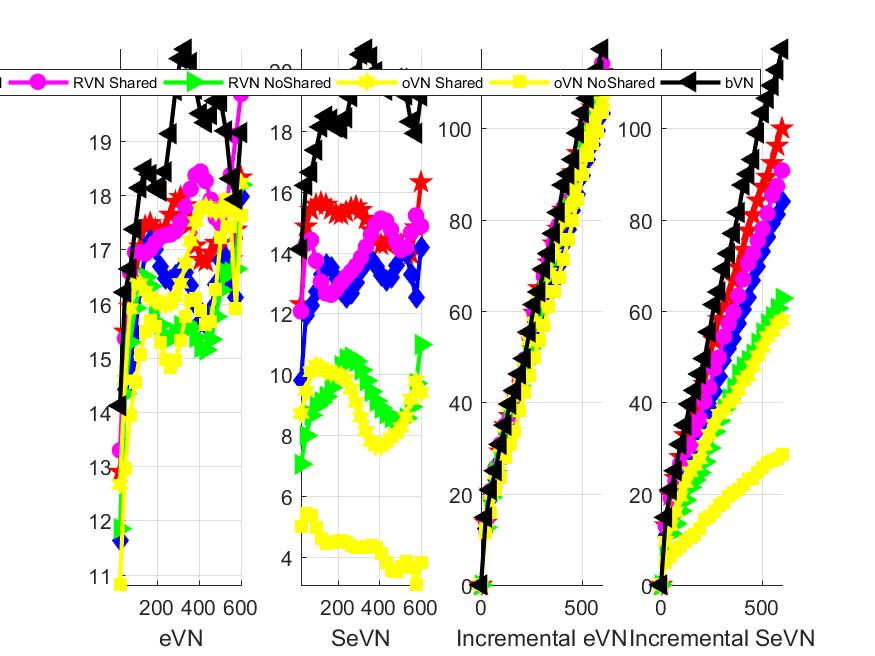
\includegraphics[width=3in]{Fig/VirNetReqSurNetReq}\\
  \caption{Accepted VNRs and Accepted SeVNRs}\label{fig:VirNetReqSurNetReq}
\end{figure}

\begin{itemize}
  \item \textbf{Acceptance Ratio}: Opposite to the concept of Blocking Probability. Ratio of a virtual network request is successful embedded into physical network denoted as $A_{eVN}/A_{VN}$. Ratio of embedded virtual networks that were successfully added for survivable guarantees and embedded into the physical topology denoted as $A_{SeVN}/A_{VN}$. Ratio of a embedded virtual network is successful survivable when the virtual network had been embedded in physical network denoted as $A_{SeVN}/A_{eVN}$.
  \item \textbf{Active Node}, represent that number of physical network booted nodes and number of survivable embedded virtual network request demand nodes. This metric is especially useful in the context of energy efficient VNE algorithms.
  \item \textbf{Path Length}: the path length metric measures the number of links between two interconnected virtual nodes, the number of links between two physical nodes that are mapped to two interconnected virtual nodes.

  \item \textbf{Cost, Revenue, and Cost/Revenue}: Cost: Sum of node computing ability or link bandwidth resources being used for the embedding. Revenue: Sum of node computing ability or link bandwidth demands realized for the virtual networks. Cost/Revenue: The ratio indicates the virtualization overhead.
  \item \textbf{Stress}: Average number of virtual links/nodes that have been assigned to the physical links/nodes .
 \item \textbf{Migration Frequency Ratio}: The number of migrations refers to the number of virtual nodes that need to be migrated to new facility nodes in case corresponding physical nodes fail.
 \item \textbf{Utilization}: Bandwidth utilization or computing utilization of physical links/nodes, in each SN entity (node or link), the sum of the spent physical resources due to the mapping of virtual entities divided by the total amount of resources.
 \item \textbf{Backup nodes number}: The number of backups metric counts the number of backup resources that are set up for a virtual entity. Several additional physical entities can be reserved to serve as a replacement in case the entity hosting the virtual entity fails.
\end{itemize}
%\begin{table*}
%\label{tab:measure}
%  \centering
%  \begin{tabular}{ll}
%    \fbox{Accepted SeVN Ratio} & Ratio of embedded virtual networks that were successfully added and embedded into the physical topology \\
%    \fbox{Stress} & NO Average number of virtual links/nodes that have been assigned to the physical links/nodes \\
%    \fbox{Utilization}& Bandwidth/CPU utilization of physical links/nodes.\\
%    \fbox{Cost, Revenue, and Cost/Revenue}& Cost: Sum of CPU and bandwidth resources being used for the embedding. Revenue: Sum of CPU and bandwidth demands realized for the virtual networks. Cost/Revenue: The ratio indicates the virtualization overhead.\\
%    \fbox{Active Nodes} &Number of nodes that need to be active in order to host all the virtual networks. This metric is especially useful in the context of energy efficient VNE algorithms.\\
%    Path Length & NO Length of communication paths assigned to virtual links\\

%    Power Consumption &Power consumption of all Active nodes. Several power consumption models are implemented.\\
%    Runtime & Average runtime of the algorithm.\\
%    Initialization Overhead &Some algorithms come with initialization cost (in terms of runtime), e.g., the distributed algorithm presented in initially partitions the network before embedding VNRs.\\
%    Hidden Hops Ratio& Ratio of hidden hops, e.g., the number of nodes only needed for forwarding packages between other nodes. Especially useful in the context of energy efficient VNE algorithms.\\
%    Communication Overhead &Communication overhead of distributed algorithms (i.e., number of messages sent between physical nodes).
%  \end{tabular}
%\end{table*}



\subsection{Acceptance Ratio}
In this section, acceptance ratio of the embedded VN's survivable request with respect to $\MyProblemAbrreviation$ problem. Moreover, the acceptance ratio of VN without survivability requirement is presented as a baseline to gauge the impact of additional amount of resources consumed for survivability on the service provisioning capability of SN.

In Fig.\ref{fig:AcceptionRatio}, acceptance ratio drops quickly before 200 time units because there are not sufficient substrate resources for the arrived VN requests. when the amount of running VN requests in system are stable after 400 time units, acceptance ratio would keep consistent. Fig.\ref{fig:AcceptionRatio} also depicts that $\MyAlgorithmMethodAbrreviation$ lead to higher acceptance ratio than $\SecondAlgorithmMethodAbrreviation$ algorithm needless of resources sharing. In particular, comparing with $\SecondAlgorithmMethodAbrreviation$-Shared, $\MyAlgorithmMethodAbrreviation$-Shared approach achieves almost 6\% improvement of acceptance ratio in the long run. Intuitively, it is the result of fact that, for $\MyAlgorithmMethodAbrreviation$-NoShared embedding, the backup node is associated with a lot of resources since it has to emulate every primary node after it fails, and so, embedding of backup node is vulnerable. However, the acceptance ratio suffers at least 6\% losses than $\MyAlgorithmMethodAbrreviation$-Shared caused by redundant resources consumption for survivability purpose.

\begin{figure}[htbp]
  \centering
  % Requires \usepackage{graphicx}
  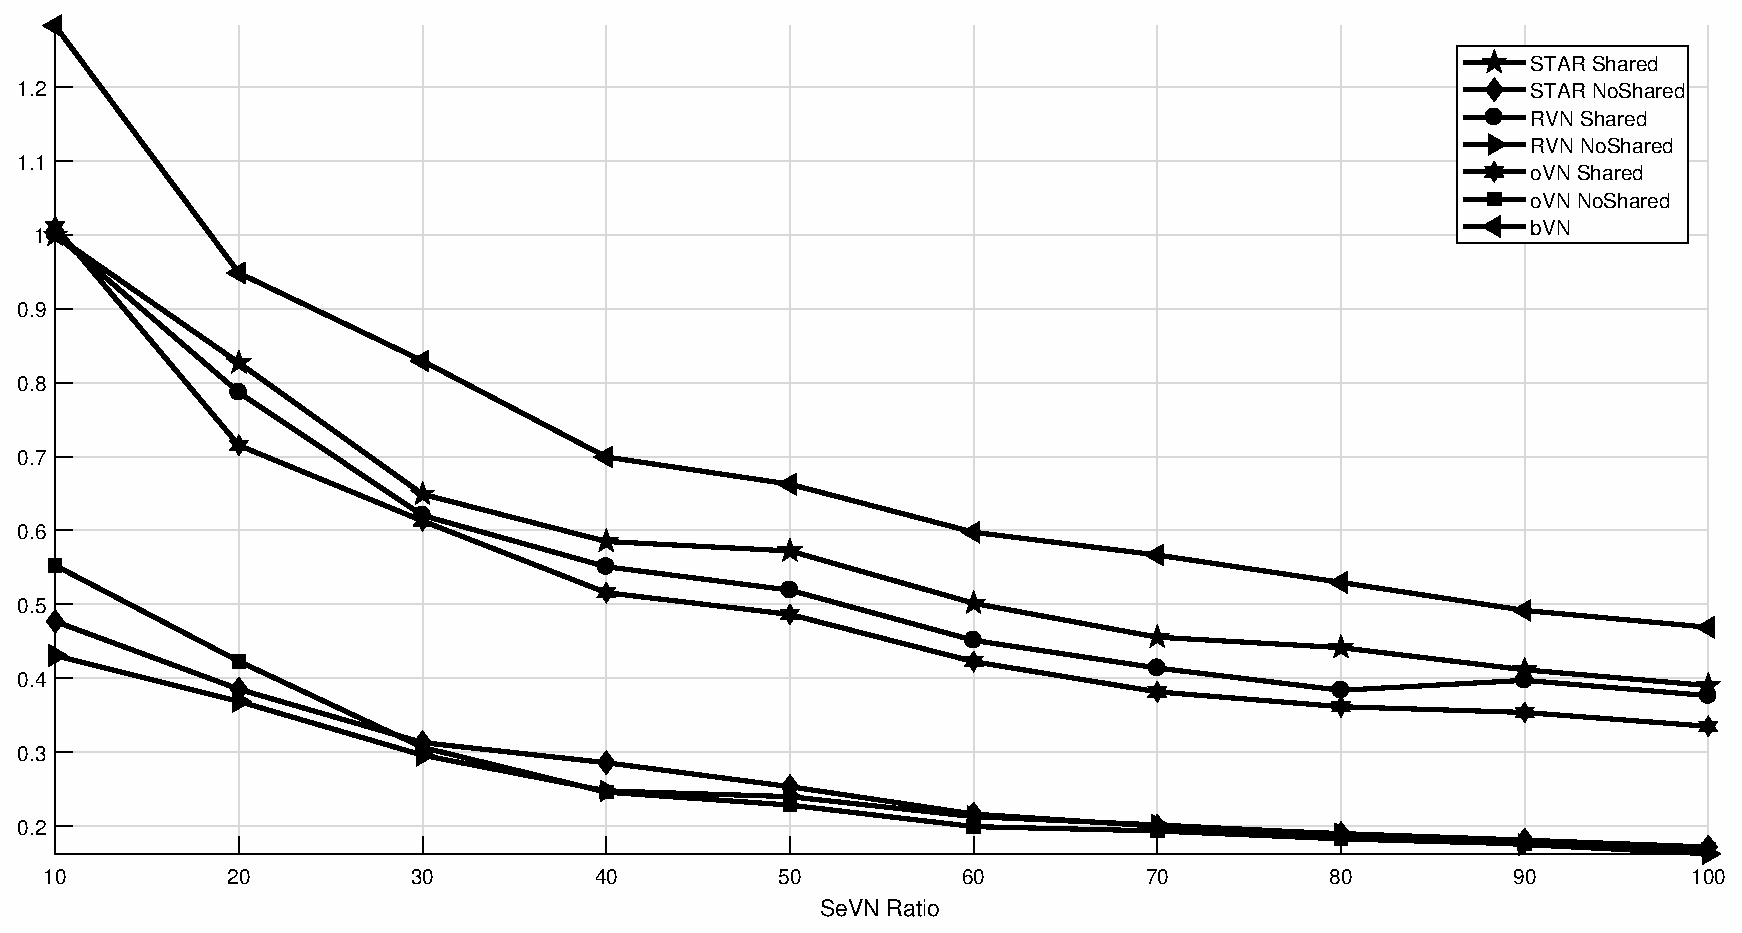
\includegraphics[width=3in]{Fig/AcceptionRatio}\\
  \caption{Acceptance Ratio}\label{fig:AcceptionRatio}
\end{figure}
\subsection{Active Node}
\subsubsection{Virtual Network Active Node}
Number of nodes that need to be active and embedded in order to host all the virtual networks.

Virtual Network Active Node Fig.\ref{fig:ActiveNodeVirtualNetwork}:
\begin{figure}[htbp]
  \centering
  % Requires \usepackage{graphicx}
  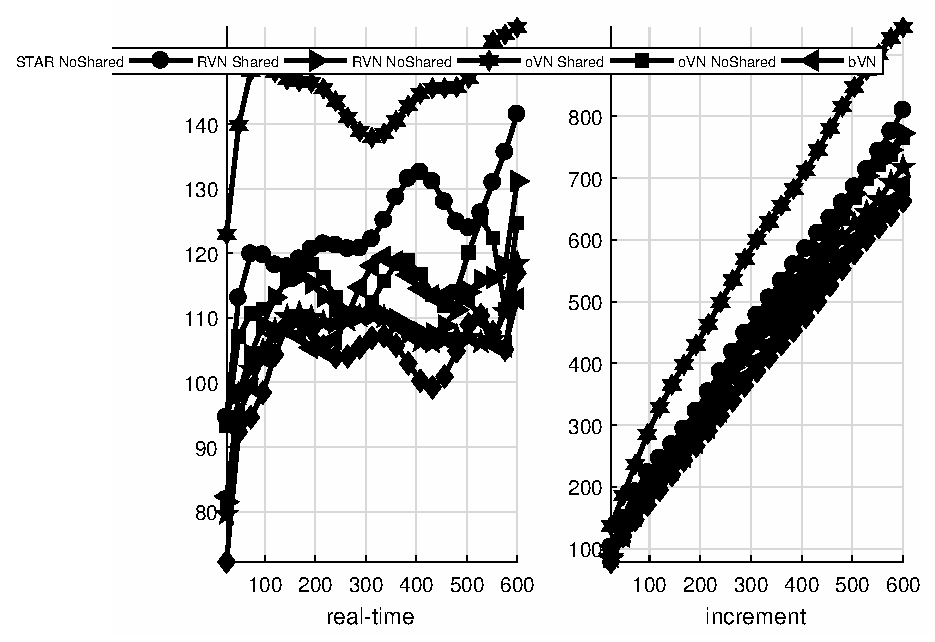
\includegraphics[width=3in]{Fig/ActiveNodeVirtualNetwork}\\
  \caption{Virtual Network Active Node}\label{fig:ActiveNodeVirtualNetwork}
\end{figure}

Virtual Network Average Active Node Fig.\ref{fig:ActiveNodeAverageVirtualNetwork}:
\begin{figure}[htbp]
  \centering
  % Requires \usepackage{graphicx}
  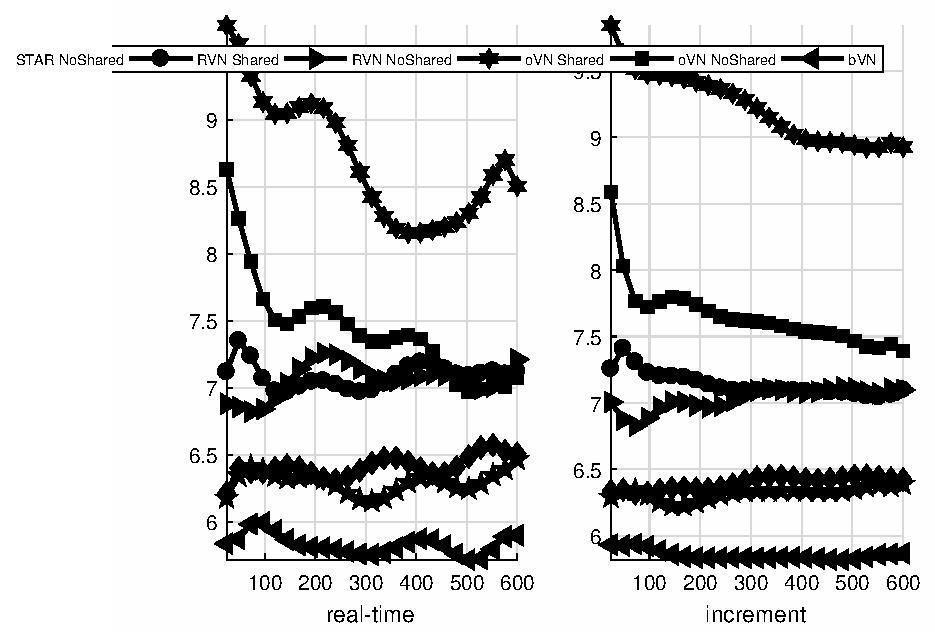
\includegraphics[width=3in]{Fig/ActiveNodeAverageVirtualNetwork}\\
  \caption{Virtual Network Average Active Node}\label{fig:ActiveNodeAverageVirtualNetwork}
\end{figure}

\subsubsection{Substrate Network Active Node}
The number of active substrate nodes is related to the average length of substrate paths, because additional nodes are used to forward communication data between end nodes. Therefore, the probability that previously switched off nodes are selected to forward data rises. Regarding energy efficiency, the number of nodes that need to be turned for an embedding can be a rough estimation of energy consumption.

Substrate Network Active Node Fig.\ref{fig:ActiveNodeSubstrateNetwork}:
\begin{figure}[htbp]
  \centering
  % Requires \usepackage{graphicx}
  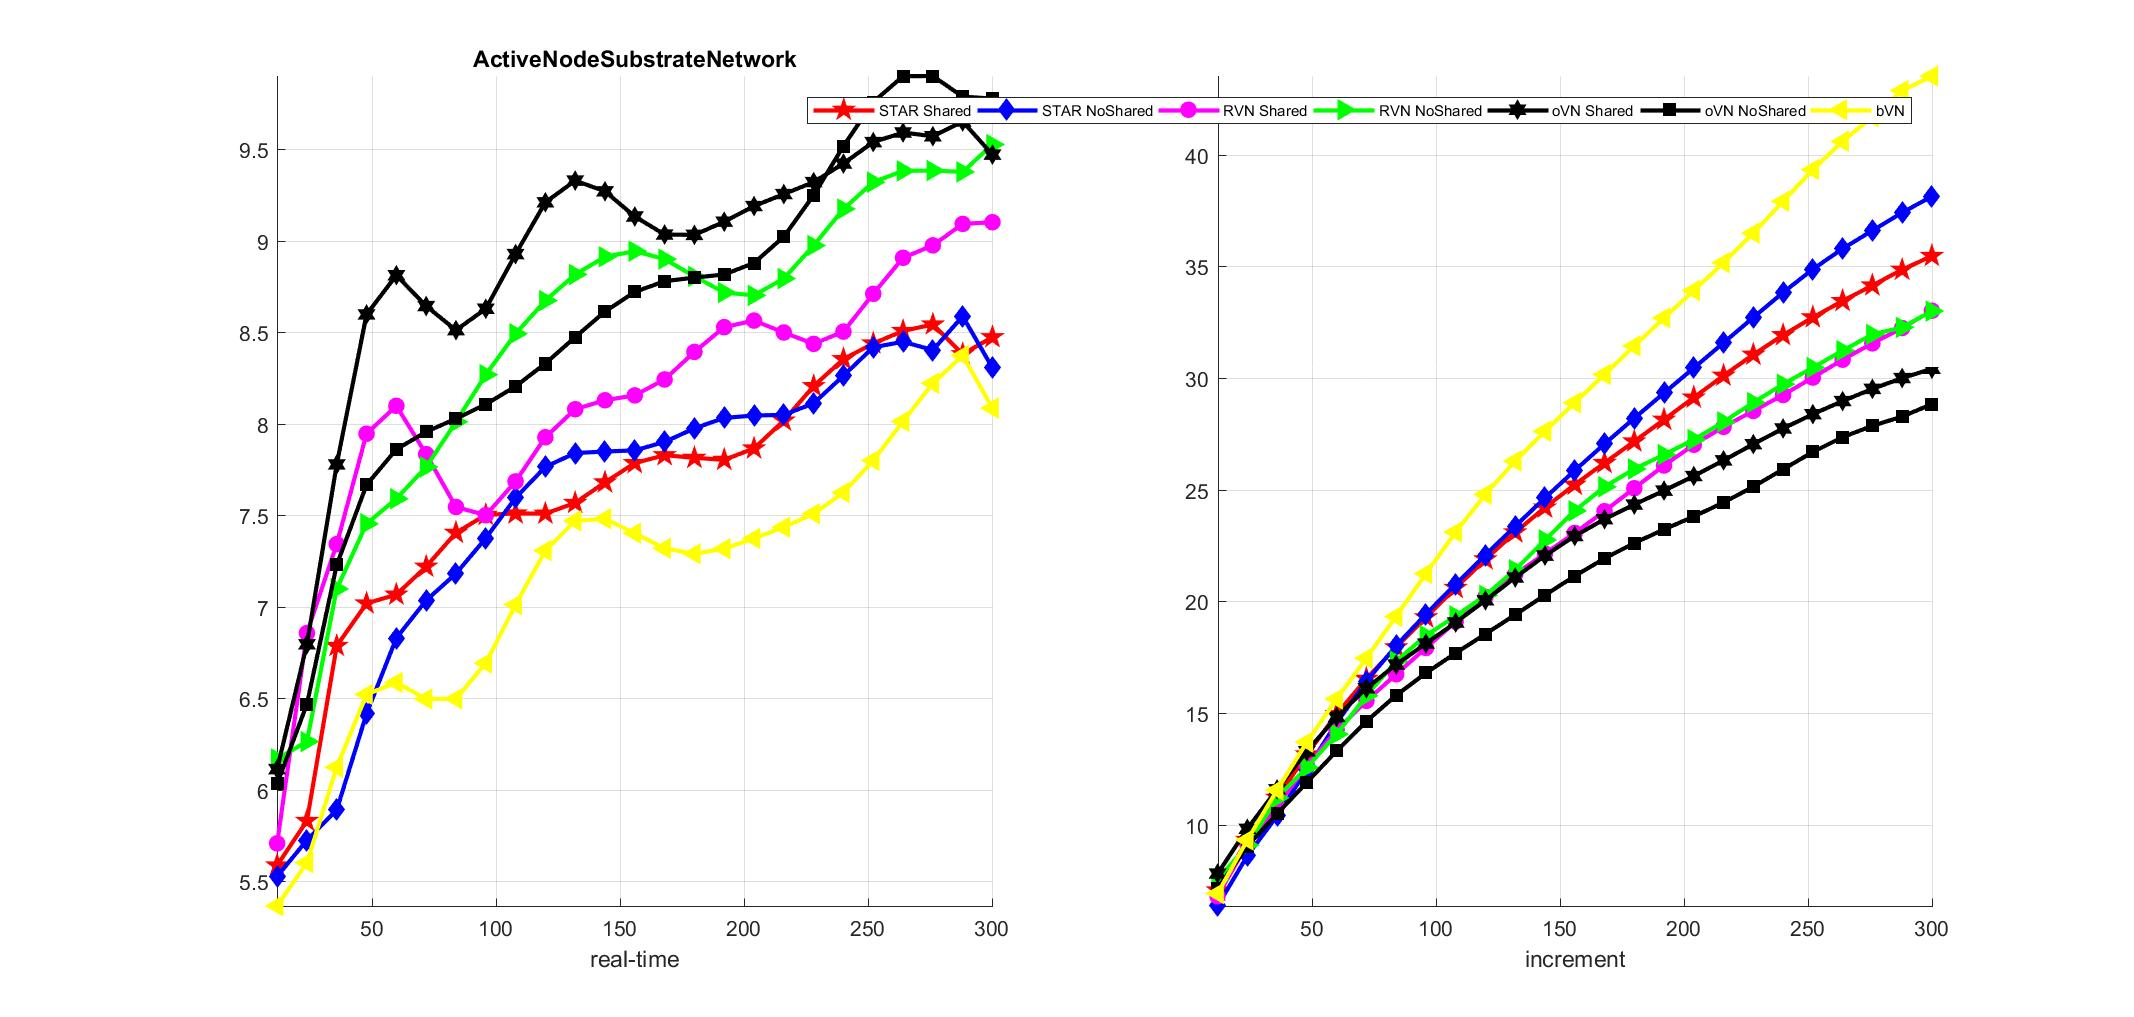
\includegraphics[width=3in]{Fig/ActiveNodeSubstrateNetwork}\\
  \caption{Substrate Network Active Node}\label{fig:ActiveNodeSubstrateNetwork}
\end{figure}


Substrate Network Average Active Node Fig.\ref{fig:ActiveNodeAverageSubstrateNetwork}:
\begin{figure}[htbp]
  \centering
  % Requires \usepackage{graphicx}
  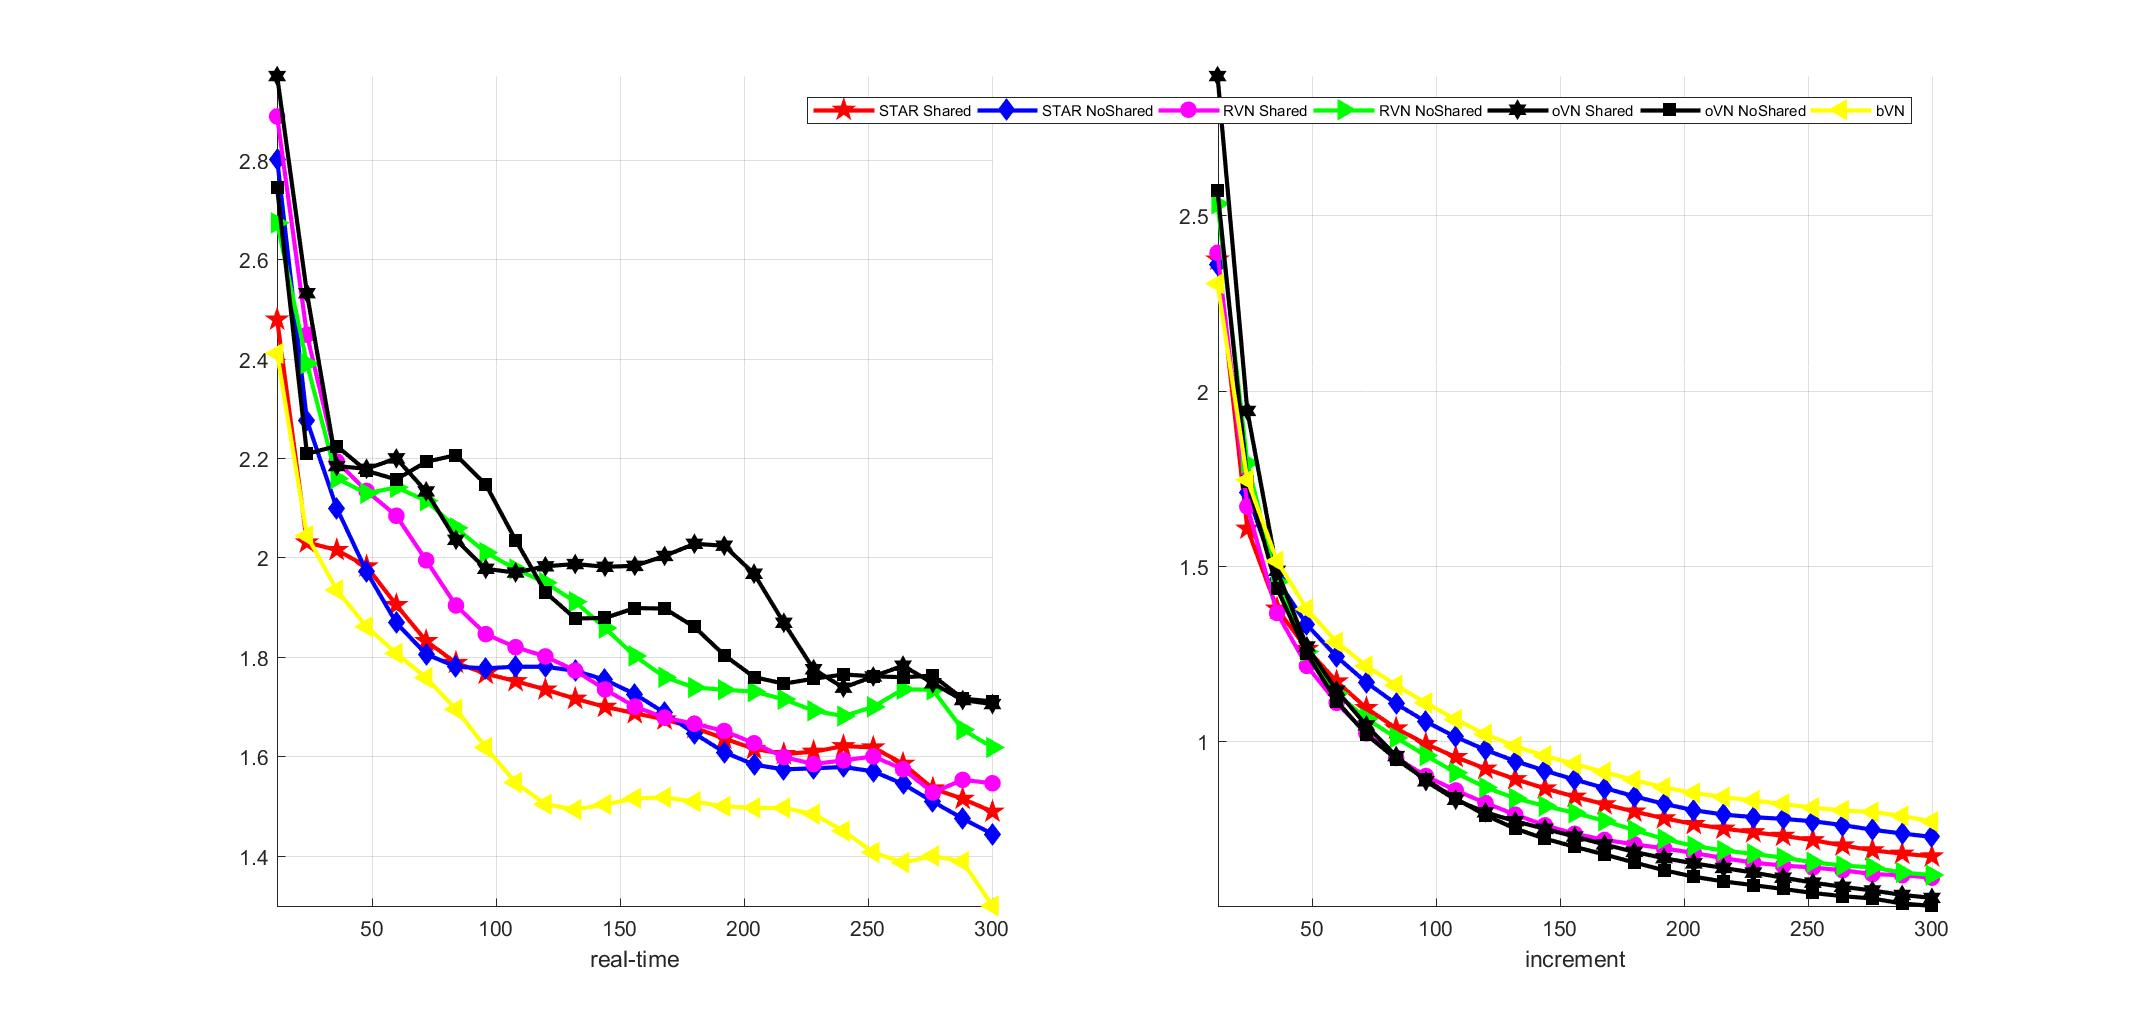
\includegraphics[width=3in]{Fig/ActiveNodeAverageSubstrateNetwork}\\
  \caption{Substrate Network Average Active Node }\label{fig:ActiveNodeAverageSubstrateNetwork}
\end{figure}

\subsubsection{Substrate Network Active Node/ Virtual Network Active Node }
In general, the ratio between running nodes and the total number of substrate nodes should be taken into account.

Substrate Network Active Node/ Virtual Network Active Node Fig.\ref{fig:ActiveNodeSubVir2VirNet}:
\begin{figure}[htbp]
  \centering
  % Requires \usepackage{graphicx}
  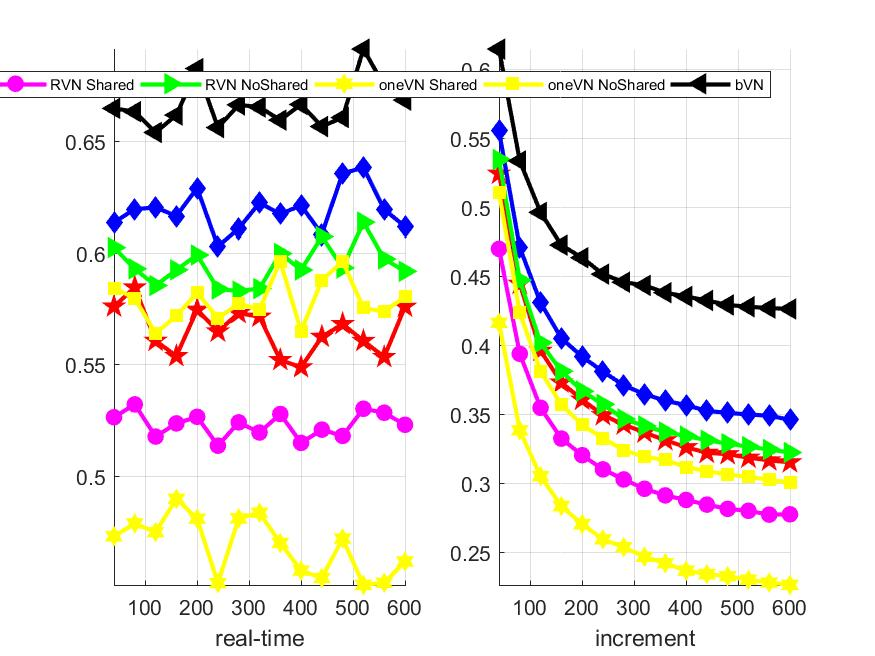
\includegraphics[width=3in]{Fig/ActiveNodeSubVir2VirNet}\\
  \caption{Substrate Network Active Node / Virtual Network Active Node}\label{fig:ActiveNodeSubVir2VirNet}
\end{figure}

\subsection{Path Length}
\subsubsection{Virtual network Path Length}

Virtual Network Path Length Fig.\ref{fig:PathLengthVirtualNetwork}
\begin{figure}[htbp]
  \centering
  % Requires \usepackage{graphicx}
  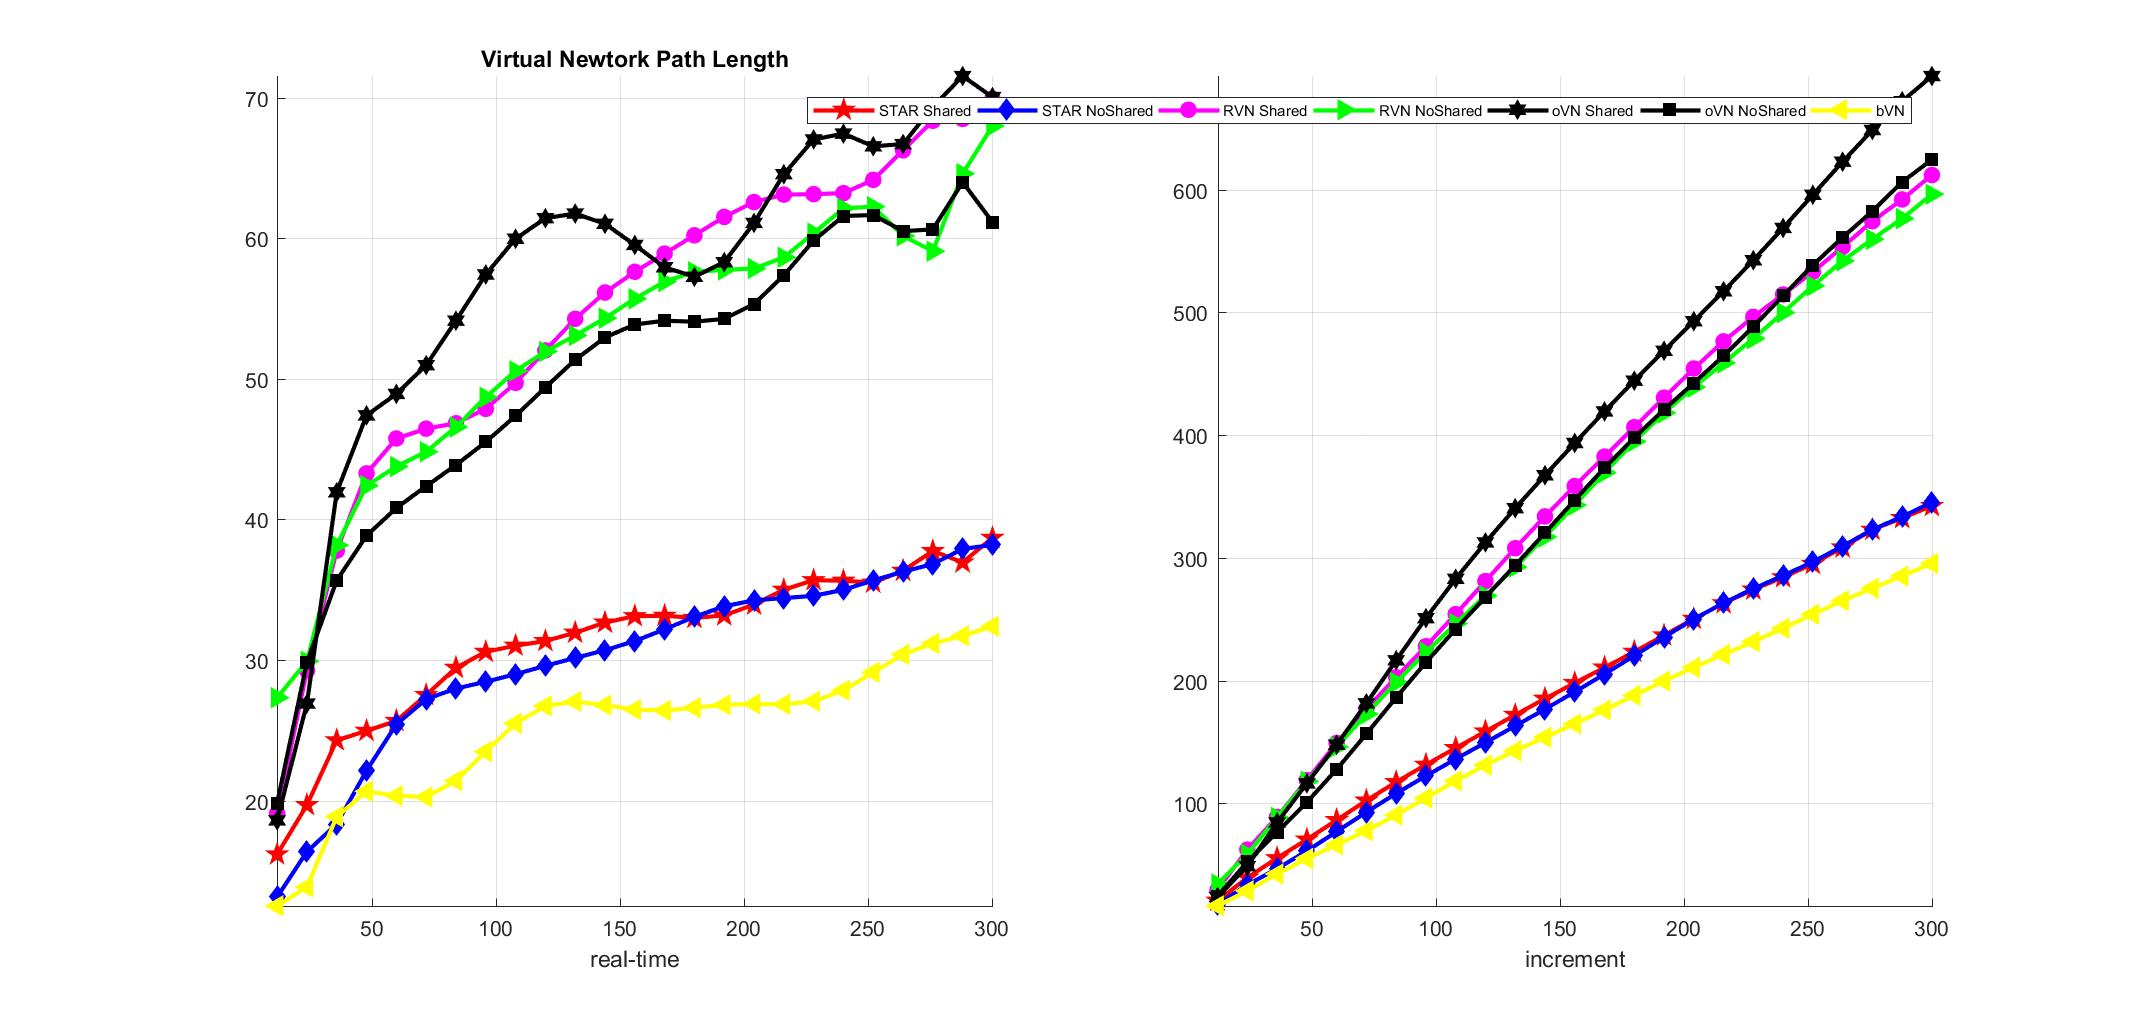
\includegraphics[width=3in]{Fig/PathLengthVirtualNetwork}\\
  \caption{ Virtual Network Path Length}\label{fig:PathLengthVirtualNetwork}
\end{figure}


Virtual Network Average Path Length Fig.\ref{fig:PathLengthAverageVirtualNetwork}:
\begin{figure}[htbp]
  \centering
  % Requires \usepackage{graphicx}
  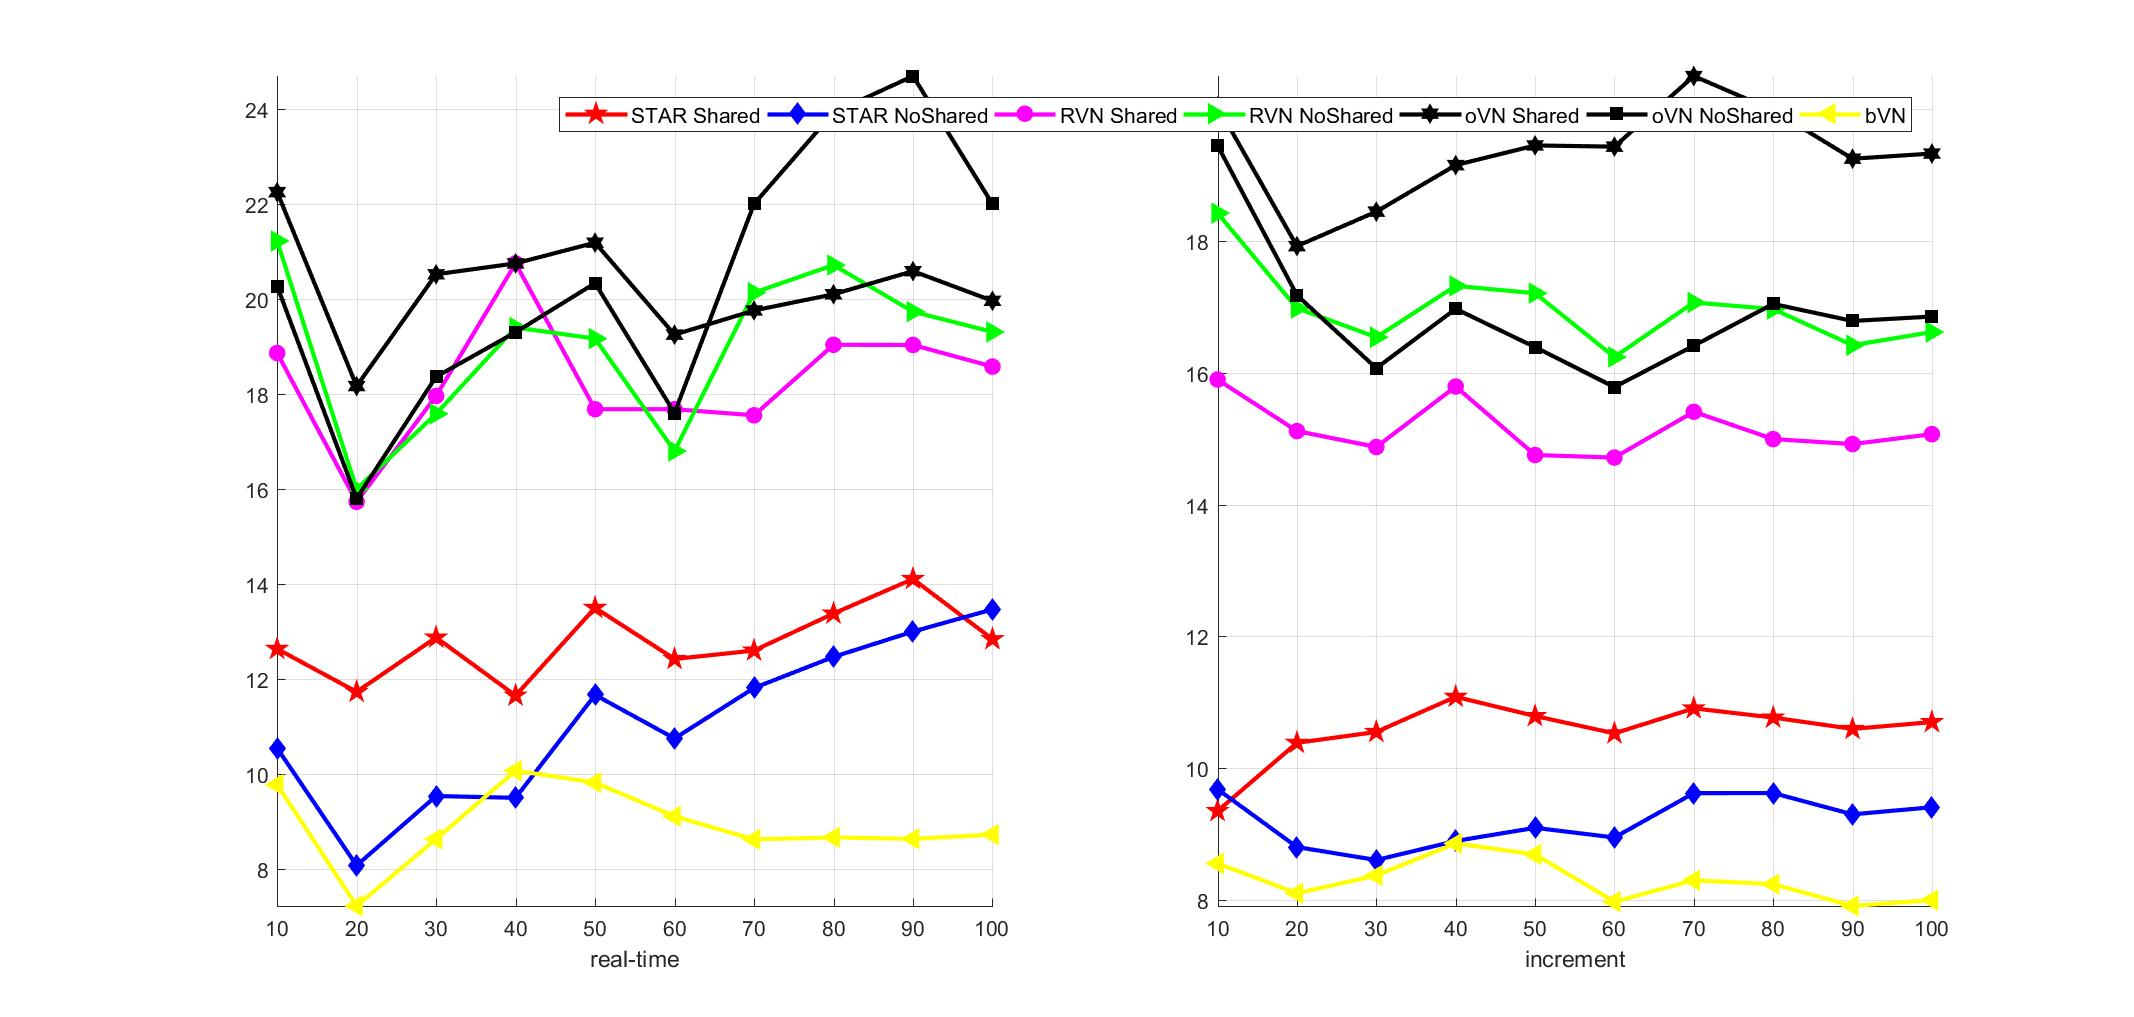
\includegraphics[width=3in]{Fig/PathLengthAverageVirtualNetwork}\\
  \caption{Virtual Network Average Path Length }\label{fig:PathLengthAverageVirtualNetwork}
\end{figure}

\subsubsection{Substrate network Path Length}
The longer a corresponding path, the more resources had to be reserved for the embedding of the virtual link. Since every substrate node (except the receiving node) that is part of a path will take some time to forward packages sent via this path, the quality of service is influenced by the path length. In general, the package delay increases in connection with the length of a path.

Substrate Network Path Length Fig.\ref{fig:PathLengthSubstrateNetwork}.
\begin{figure}[htbp]
  \centering
  % Requires \usepackage{graphicx}
  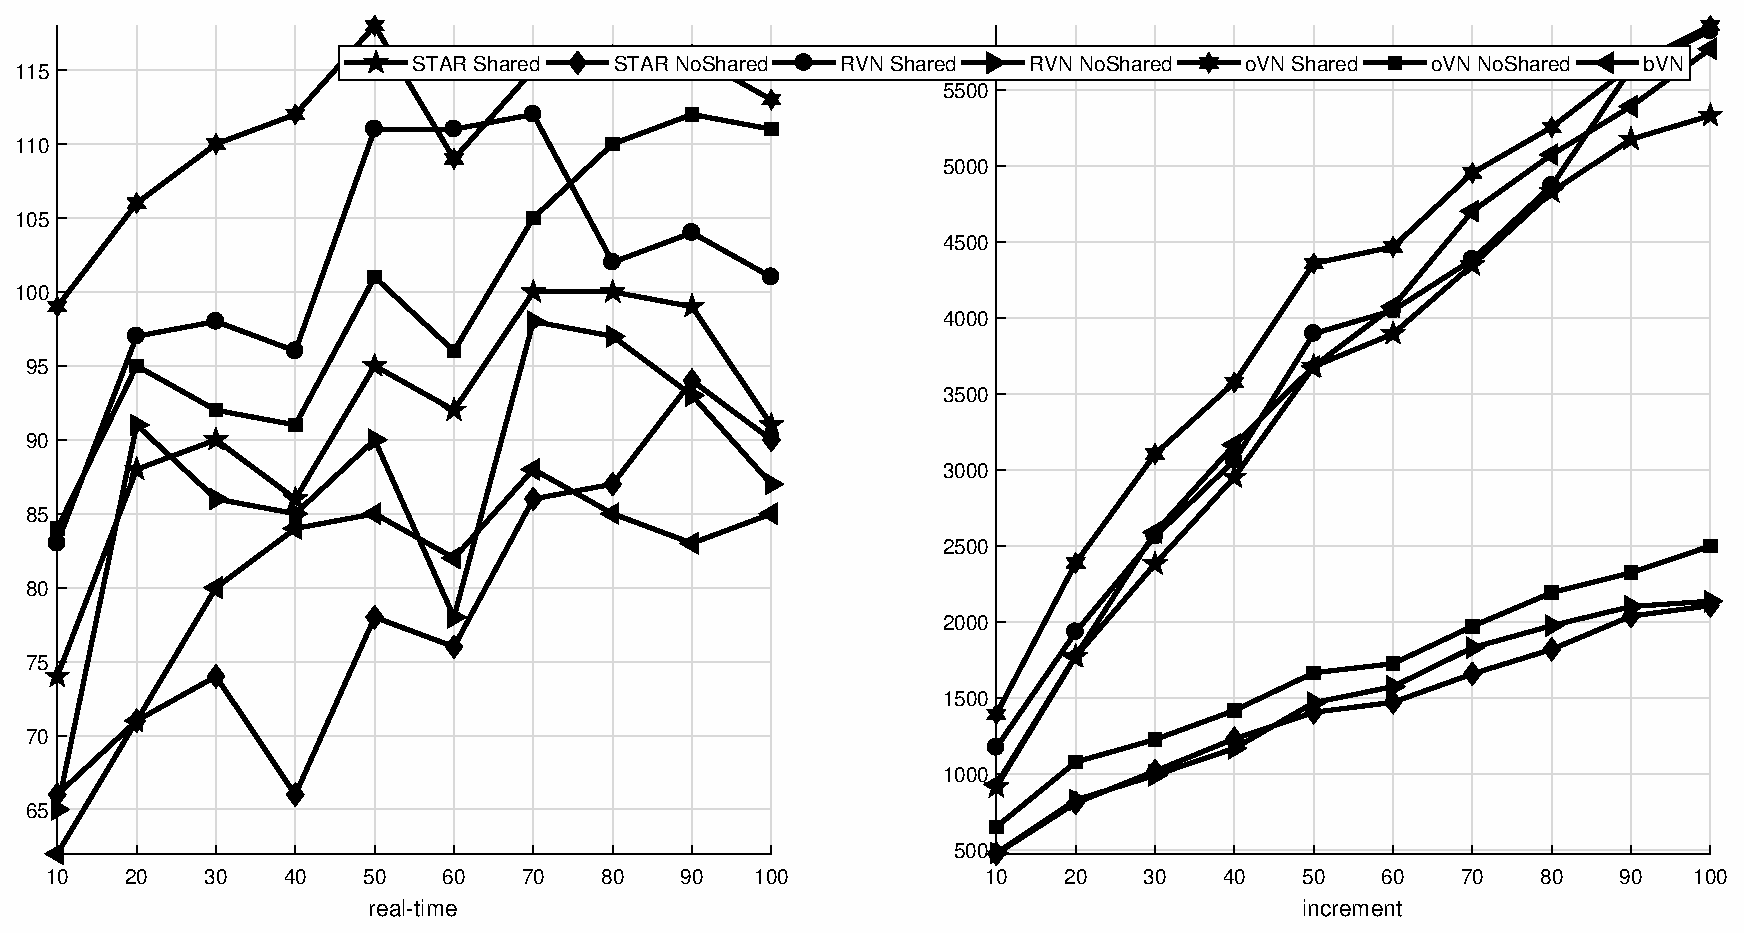
\includegraphics[width=3in]{Fig/PathLengthSubstrateNetwork}\\
  \caption{ Substrate Network Path Length}\label{fig:PathLengthSubstrateNetwork}
\end{figure}

Substrate Network Average Path Length Fig.\ref{fig:PathLengthAverageSubstrateNetwork}.
\begin{figure}[htbp]
  \centering
  % Requires \usepackage{graphicx}
  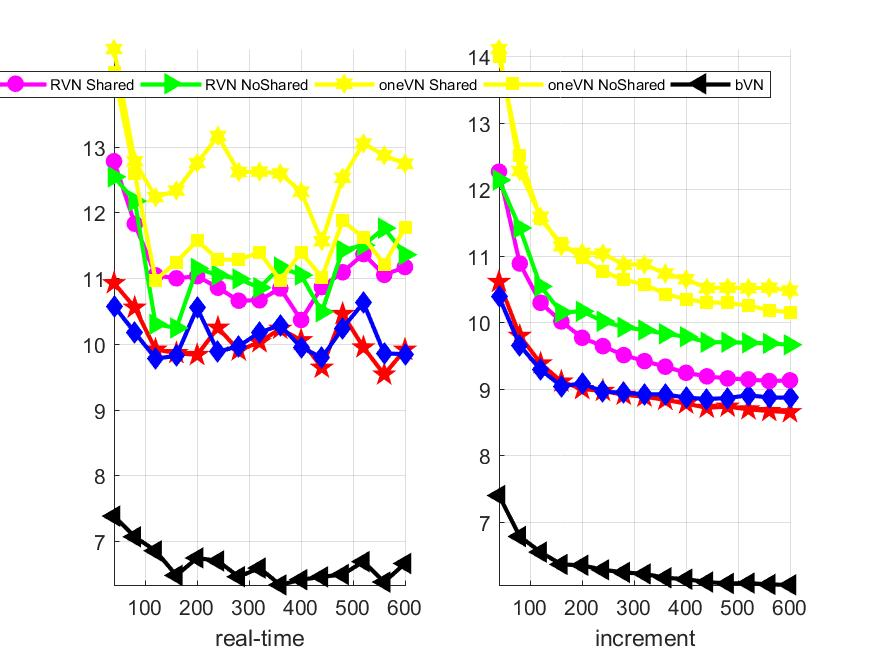
\includegraphics[width=3in]{Fig/PathLengthAverageSubstrateNetwork}\\
  \caption{ Substrate Network Average Path Length }\label{fig:PathLengthAverageSubstrateNetwork}
\end{figure}




\subsubsection{Substrate Network Path Length/ Virtual Network Path Length}


Substrate Network Path Length/ Virtual Network Path Length Fig.\ref{fig:PathLengthSubVir2VirNet}:
\begin{figure}[htbp]
  \centering
  % Requires \usepackage{graphicx}
  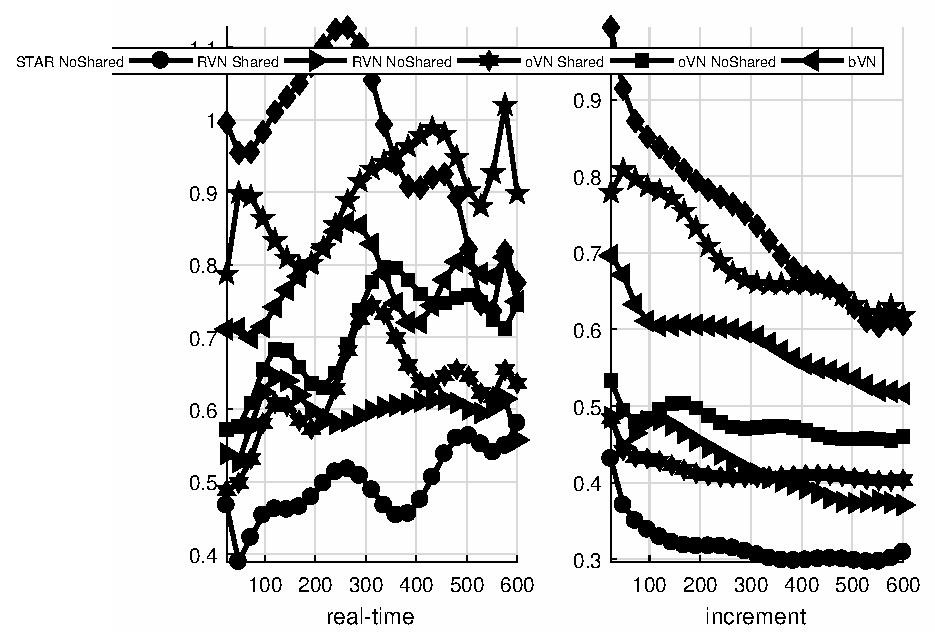
\includegraphics[width=3in]{Fig/PathLengthSubVir2VirNet}\\
  \caption{Substrate Network Path Length/ Virtual Network Path Length }\label{fig:PathLengthSubVir2VirNet}
\end{figure}



\subsection{Cost, Revenue and Cost/Revenue}
\subsubsection{Cost}
In this work, the embedding cost is calculated as the cost of the substrate resources (i.e. cost of node computing ability on all facility nodes, edge bandwidth on all fiber links) consumed to satisfy the $\MyProblemAbrreviation$ resource requirements.

Substrate Network Real-Time Cost Fig.\ref{fig:CostCurrentSubstrateNetwork}:
\begin{figure}[htbp]
  \centering
  % Requires \usepackage{graphicx}
  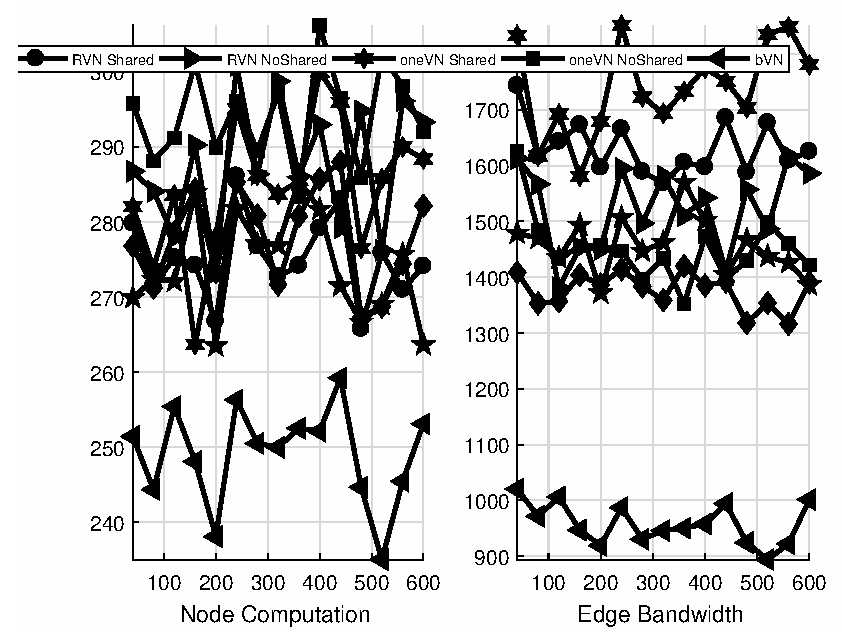
\includegraphics[width=3in]{Fig/CostCurrentSubstrateNetwork}\\
  \caption{Substrate Network Real-Time Cost}\label{fig:CostCurrentSubstrateNetwork}
\end{figure}

Substrate Network Increment Cost Fig.\ref{fig:CostAccumulateSubstrateNetwork}:
\begin{figure}[htbp]
  \centering
  % Requires \usepackage{graphicx}
  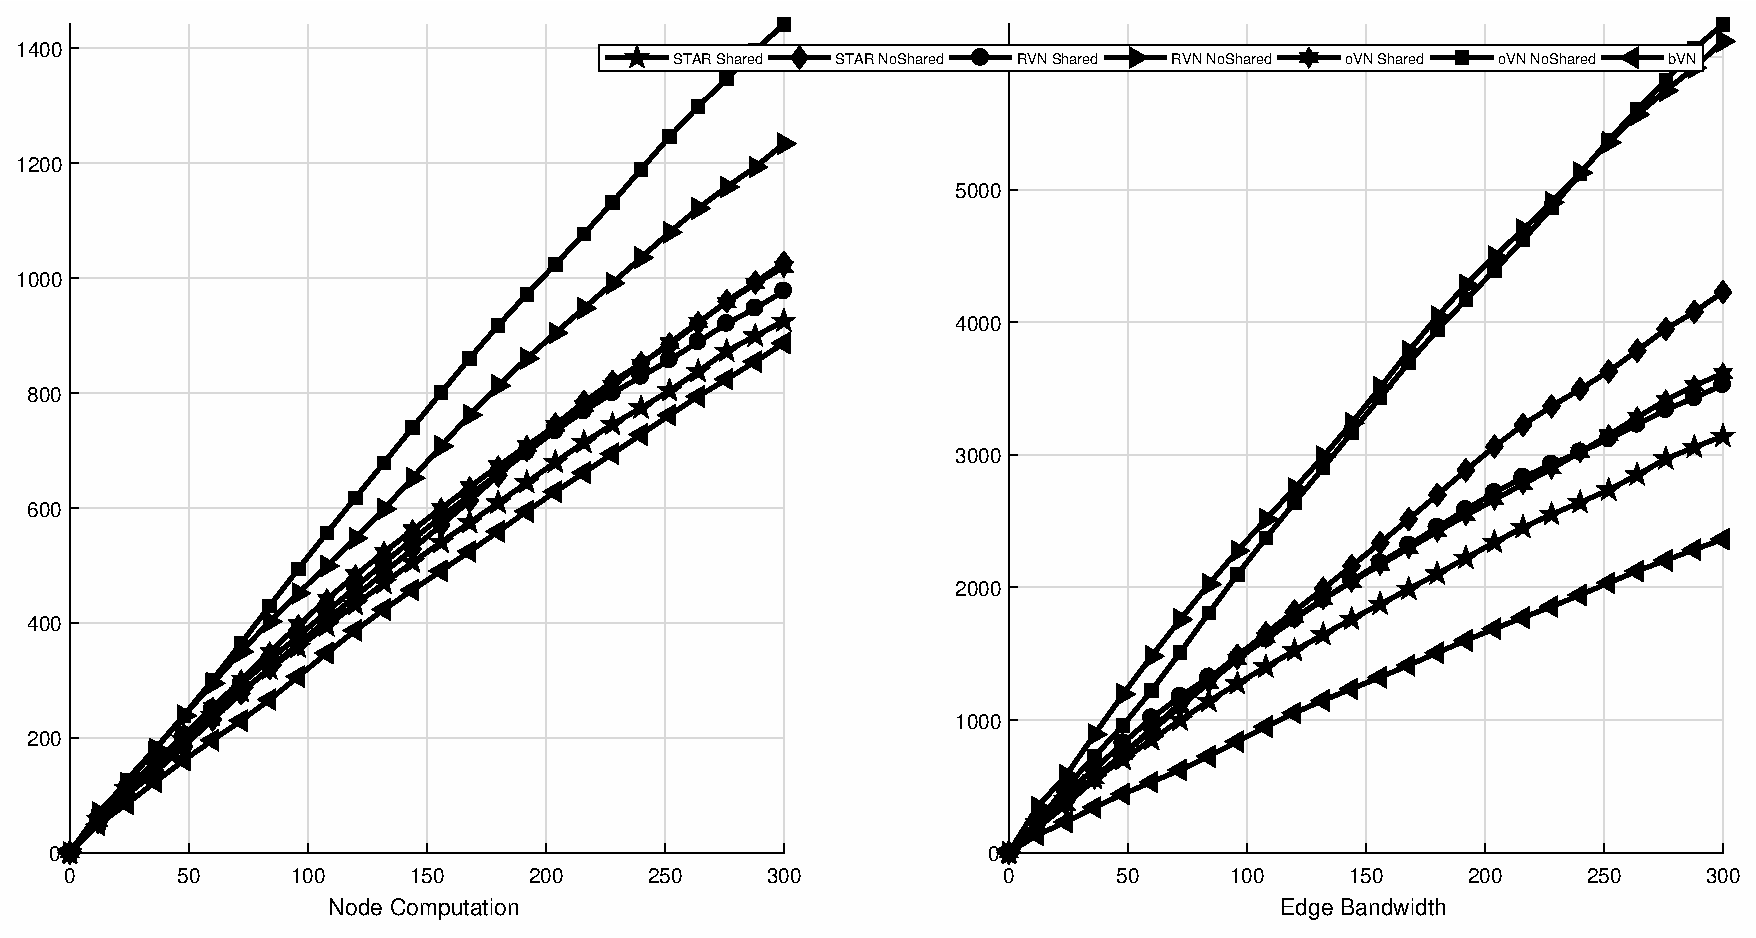
\includegraphics[width=3in]{Fig/CostAccumulateSubstrateNetwork}\\
  \caption{Substrate Network Increment Cost}\label{fig:CostAccumulateSubstrateNetwork}
\end{figure}

Substrate Network Average Real-Time  Cost Fig.\ref{fig:CostCurrentAverageSubstrateNetwork}:
\begin{figure}[htbp]
  \centering
  % Requires \usepackage{graphicx}
  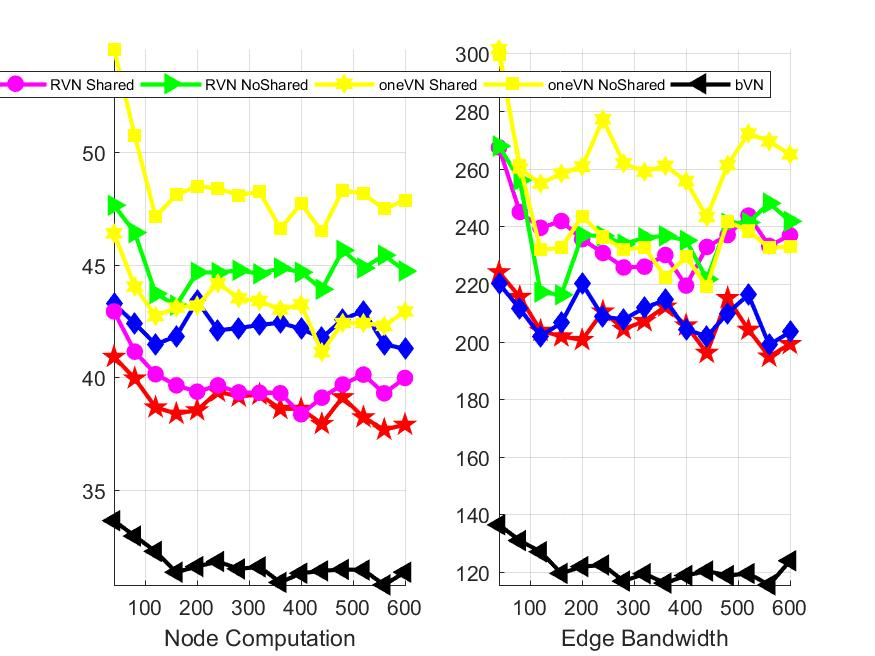
\includegraphics[width=3in]{Fig/CostCurrentAverageSubstrateNetwork}\\
  \caption{Substrate Network Average Real-Time Cost}\label{fig:CostCurrentAverageSubstrateNetwork}
\end{figure}

Substrate Network Increment Average Cost Fig.\ref{fig:CostAccumulateAverageSubstrateNetwork}:
\begin{figure}[htbp]
  \centering
  % Requires \usepackage{graphicx}
  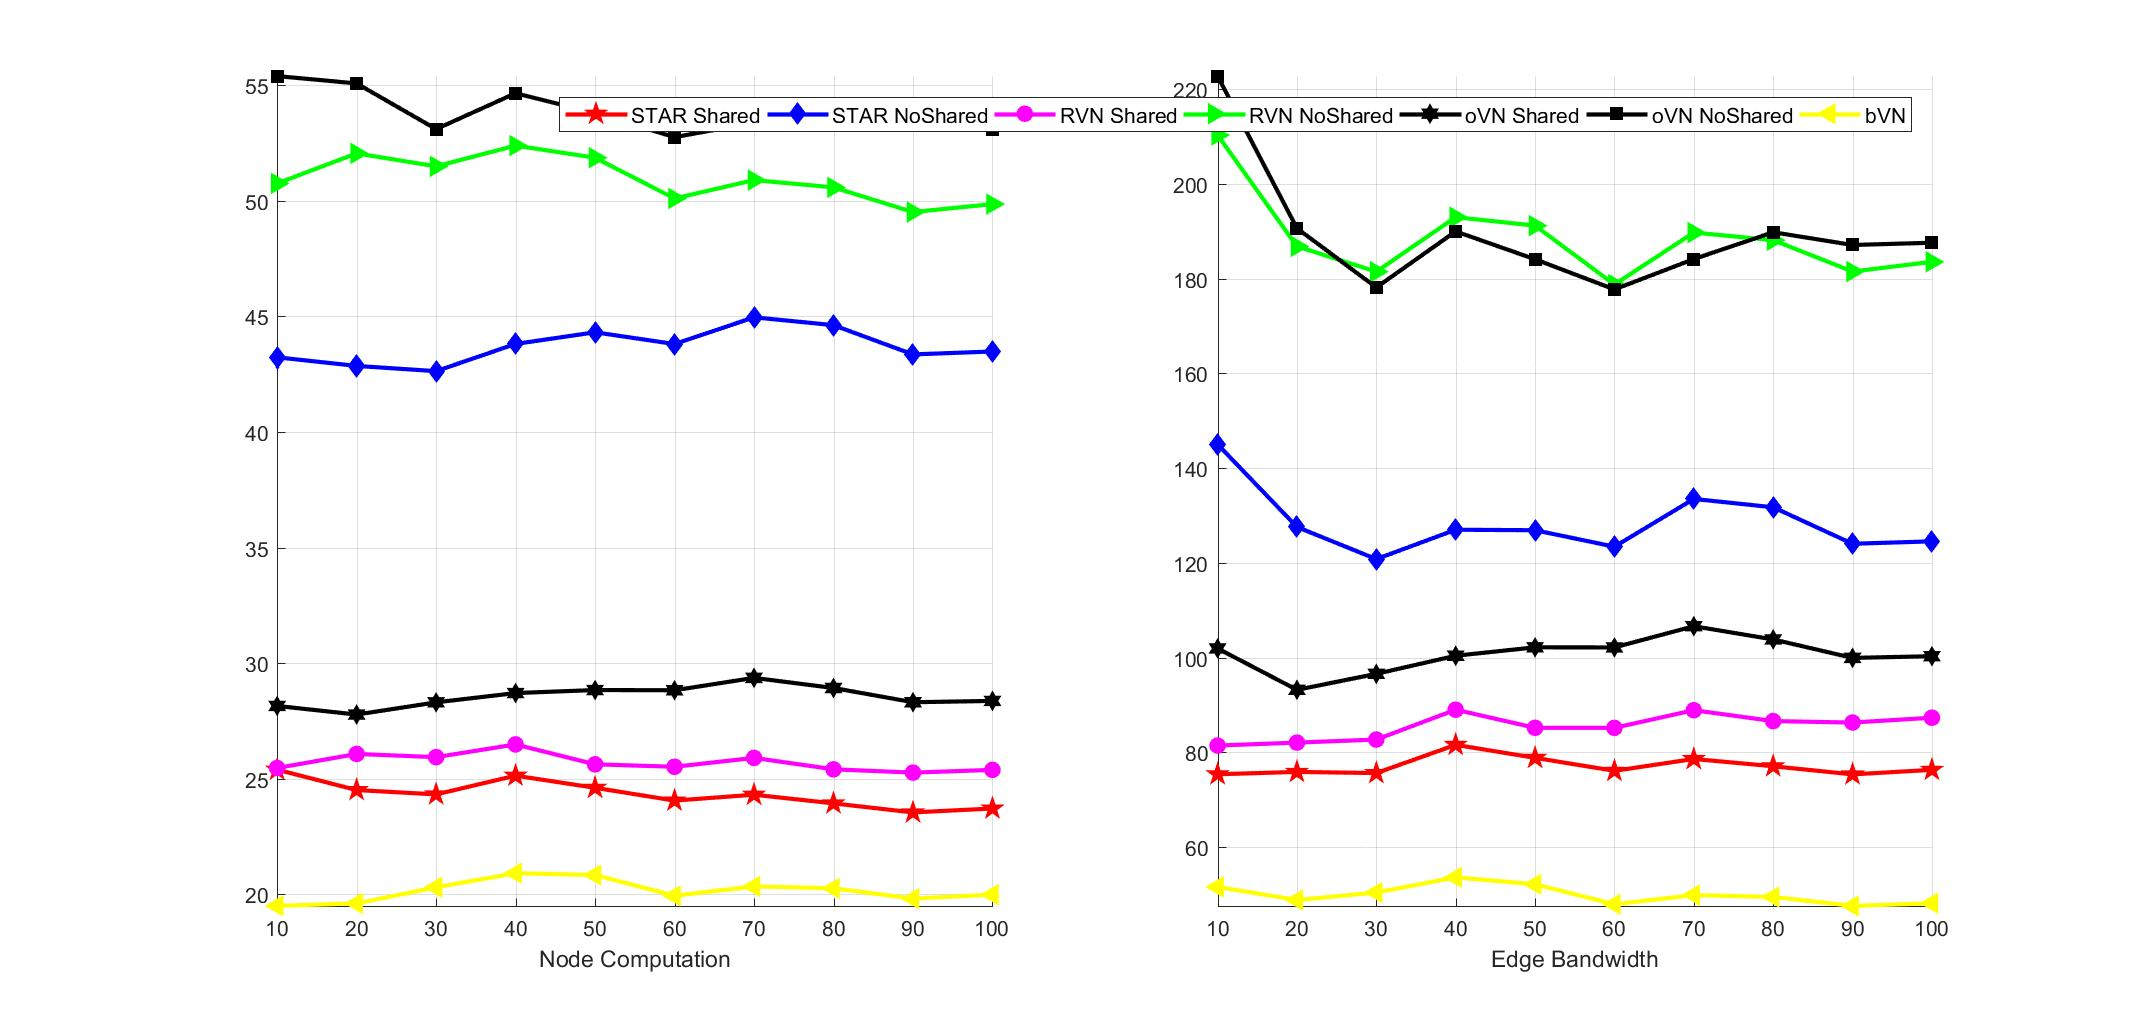
\includegraphics[width=3in]{Fig/CostAccumulateAverageSubstrateNetwork}\\
  \caption{Substrate Network Average Increment Cost }\label{fig:CostAccumulateAverageSubstrateNetwork}
\end{figure}



\subsubsection{Revenue}
Virtual Network Real-Time Revenue Fig.\ref{fig:RevenueCurrentVirtualNetwork}:
\begin{figure}[htbp]
  \centering
  % Requires \usepackage{graphicx}
  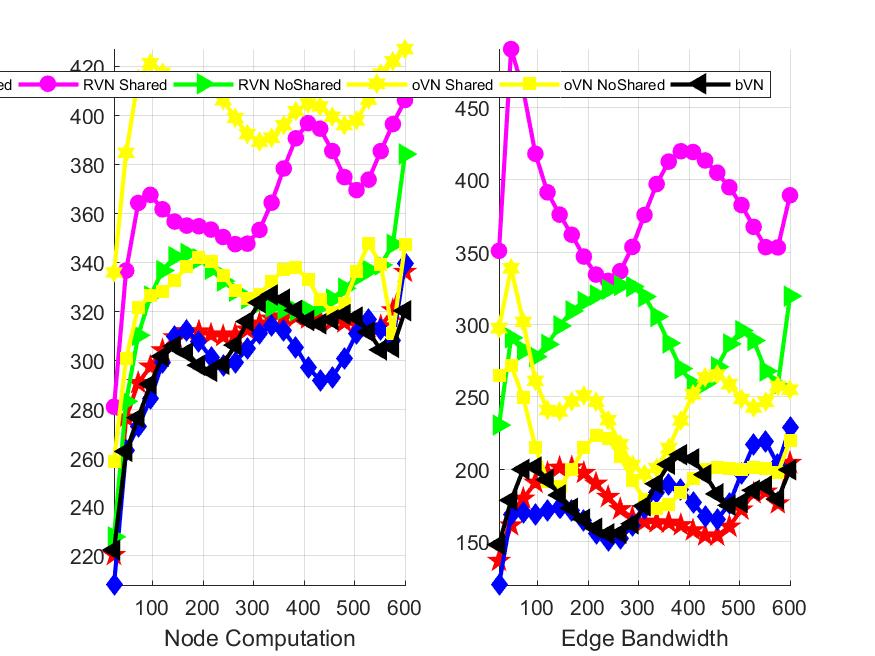
\includegraphics[width=3in]{Fig/RevenueCurrentVirtualNetwork}\\
  \caption{Virtual Network Real-Time Revenue }\label{fig:RevenueCurrentVirtualNetwork}
\end{figure}

Virtual Network Increment Revenue Fig.\ref{fig:RevenueAccumulateVirtualNetwork}:
\begin{figure}[htbp]
  \centering
  % Requires \usepackage{graphicx}
  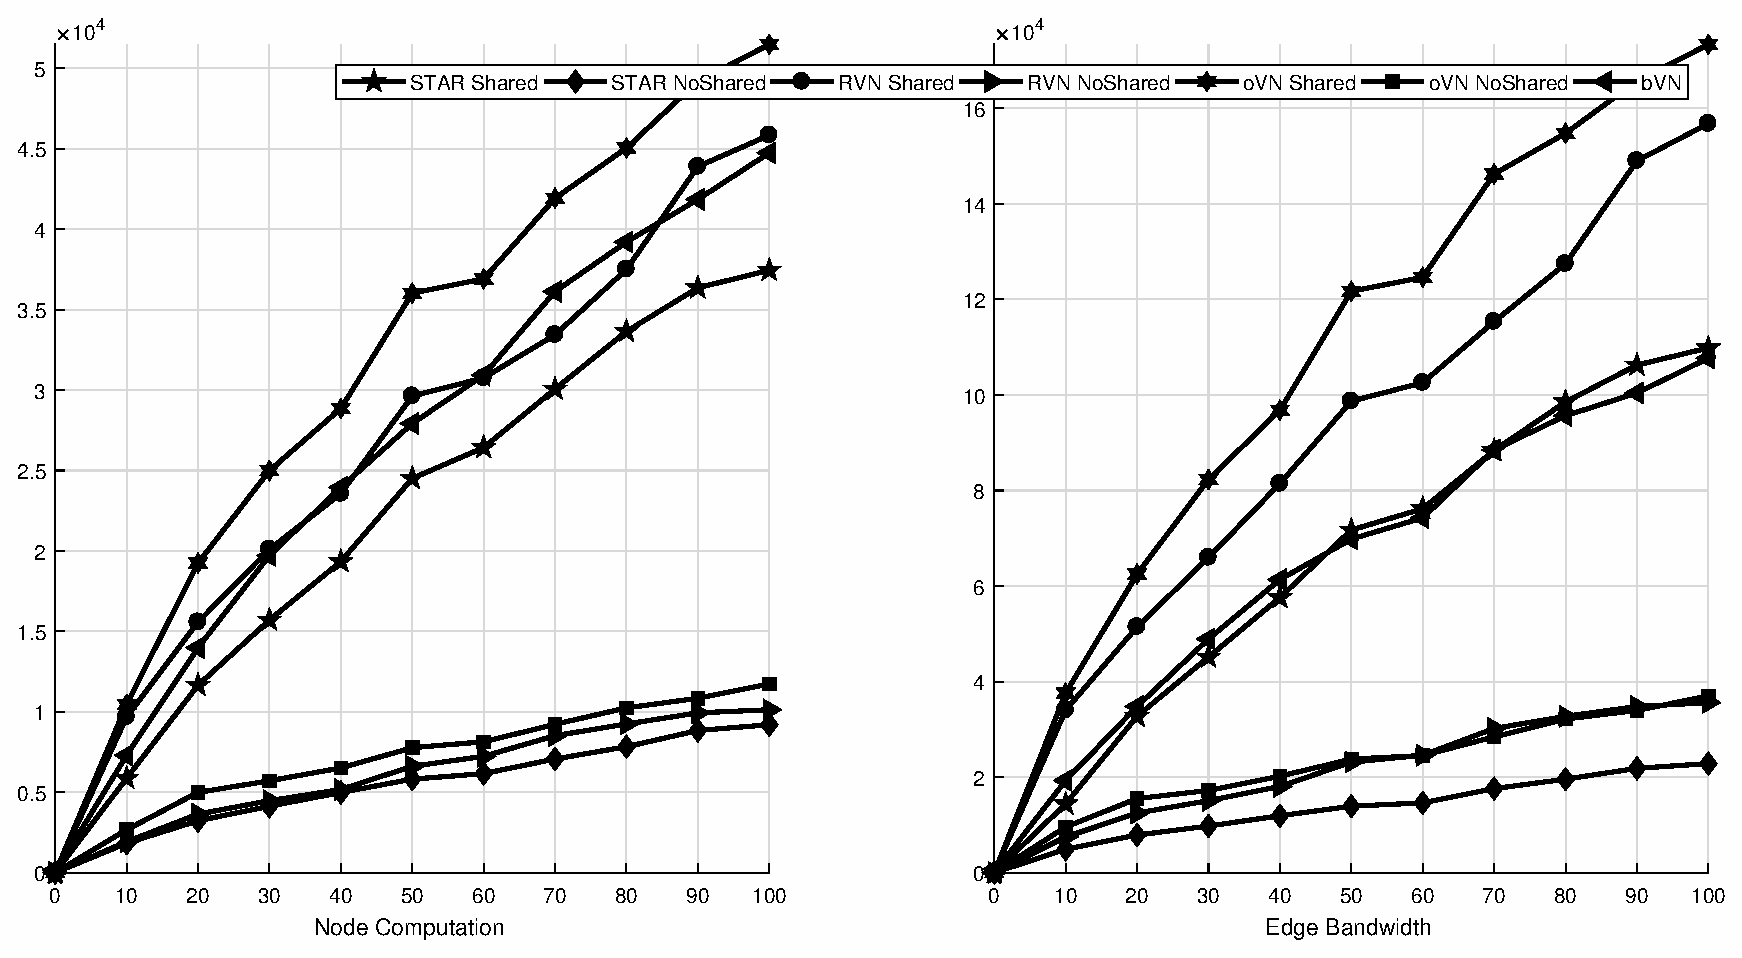
\includegraphics[width=3in]{Fig/RevenueAccumulateVirtualNetwork}\\
  \caption{Virtual Network Increment Revenue }\label{fig:RevenueAccumulateVirtualNetwork}
\end{figure}

Virtual Network Average Real-Time Revenue Fig.\ref{fig:RevenueAverageCurrentVirtualNetwork}:
\begin{figure}[htbp]
  \centering
  % Requires \usepackage{graphicx}
  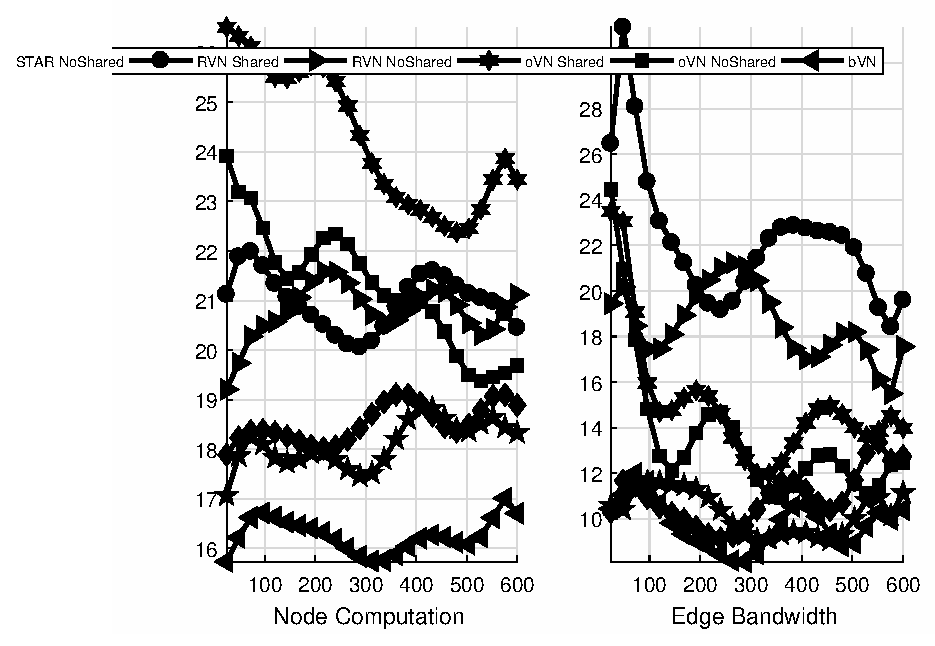
\includegraphics[width=3in]{Fig/RevenueAverageCurrentVirtualNetwork}\\
  \caption{Virtual Network Average Real-Time Revenue}\label{fig:RevenueAverageCurrentVirtualNetwork}
\end{figure}

Virtual Network Average Increment Revenue Fig.\ref{fig:RevenueAccumulateAverageVirtualNetwork}:
\begin{figure}[htbp]
  \centering
  % Requires \usepackage{graphicx}
  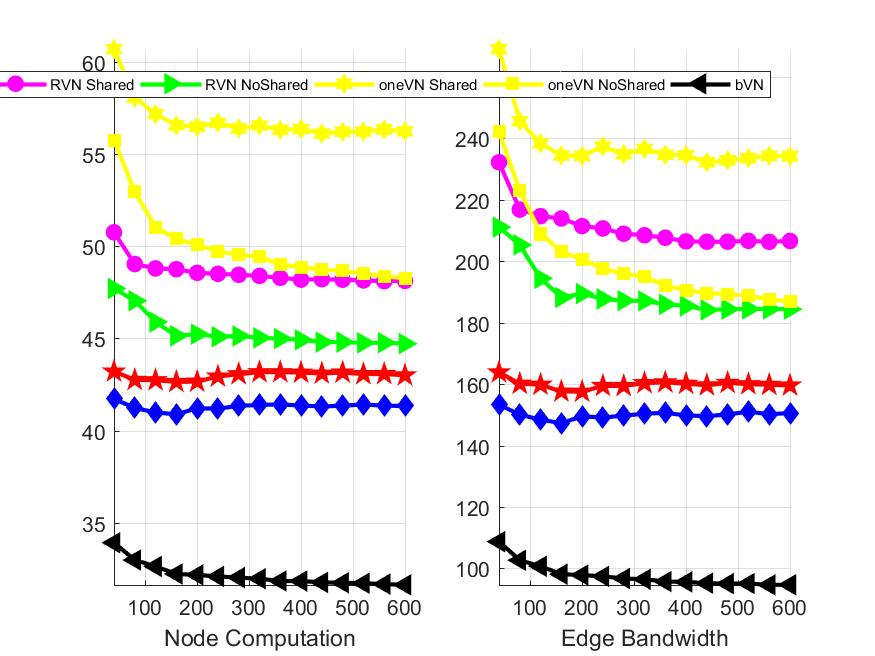
\includegraphics[width=3in]{Fig/RevenueAccumulateAverageVirtualNetwork}\\
  \caption{Virtual Network Average Increment Revenue}\label{fig:RevenueAccumulateAverageVirtualNetwork}
\end{figure}


\subsubsection{Cost/Revenue}
By dividing Cost by Revenue, varying Cost values are balanced. The higher the value, the more resources were needed to embed the SeVNs.

Cost/Revenue Fig.\ref{fig:CostRevenue}:
\begin{figure}[htbp]
  \centering
  % Requires \usepackage{graphicx}
  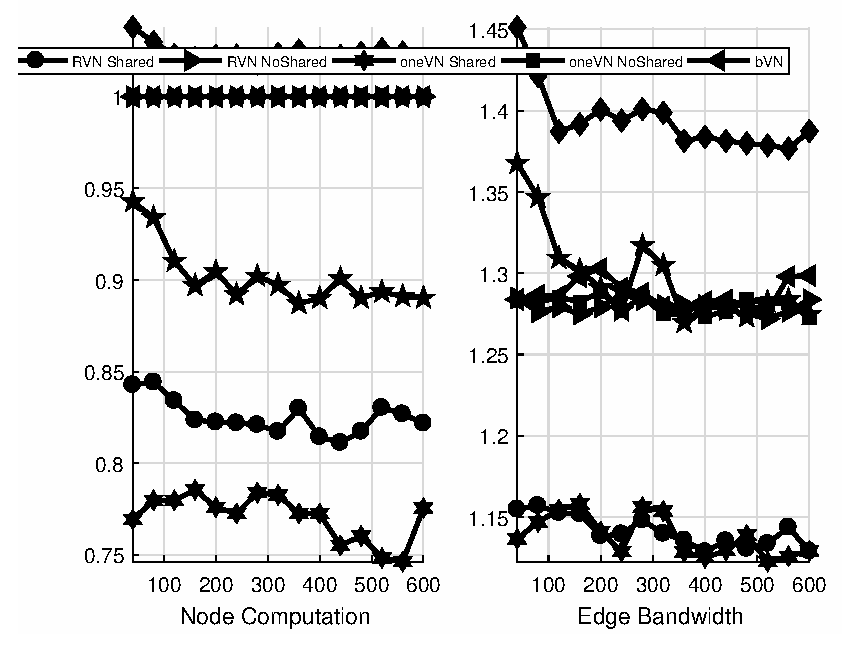
\includegraphics[width=3in]{Fig/CostRevenue}\\
  \caption{Cost/Revenue}\label{fig:CostRevenue}
\end{figure}

Increment Cost to Increment Revenue Fig.\ref{fig:CostRevenueAccumulate}:
\begin{figure}[htbp]
  \centering
  % Requires \usepackage{graphicx}
  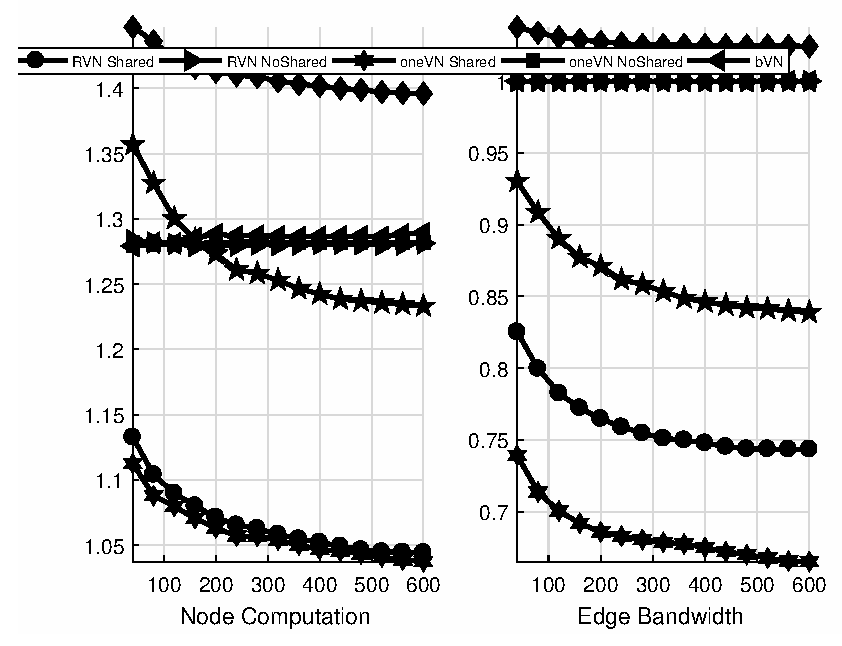
\includegraphics[width=3in]{Fig/CostRevenueAccumulate}\\
  \caption{Increment Cost/Increment Revenue}\label{fig:CostRevenueAccumulate}
\end{figure}



\subsection{Migration Frequency}
Typically, at least the virtual nodes hosted on the failing substrate nodes have to be moved. Other constraints, like maximum path length, might however trigger even more migrations. Since migrations are resource intensive, they should be kept to a minimum.
Fig.\ref{fig:MigrationFrequence}
\begin{figure}[htbp]
  \centering
  % Requires \usepackage{graphicx}
  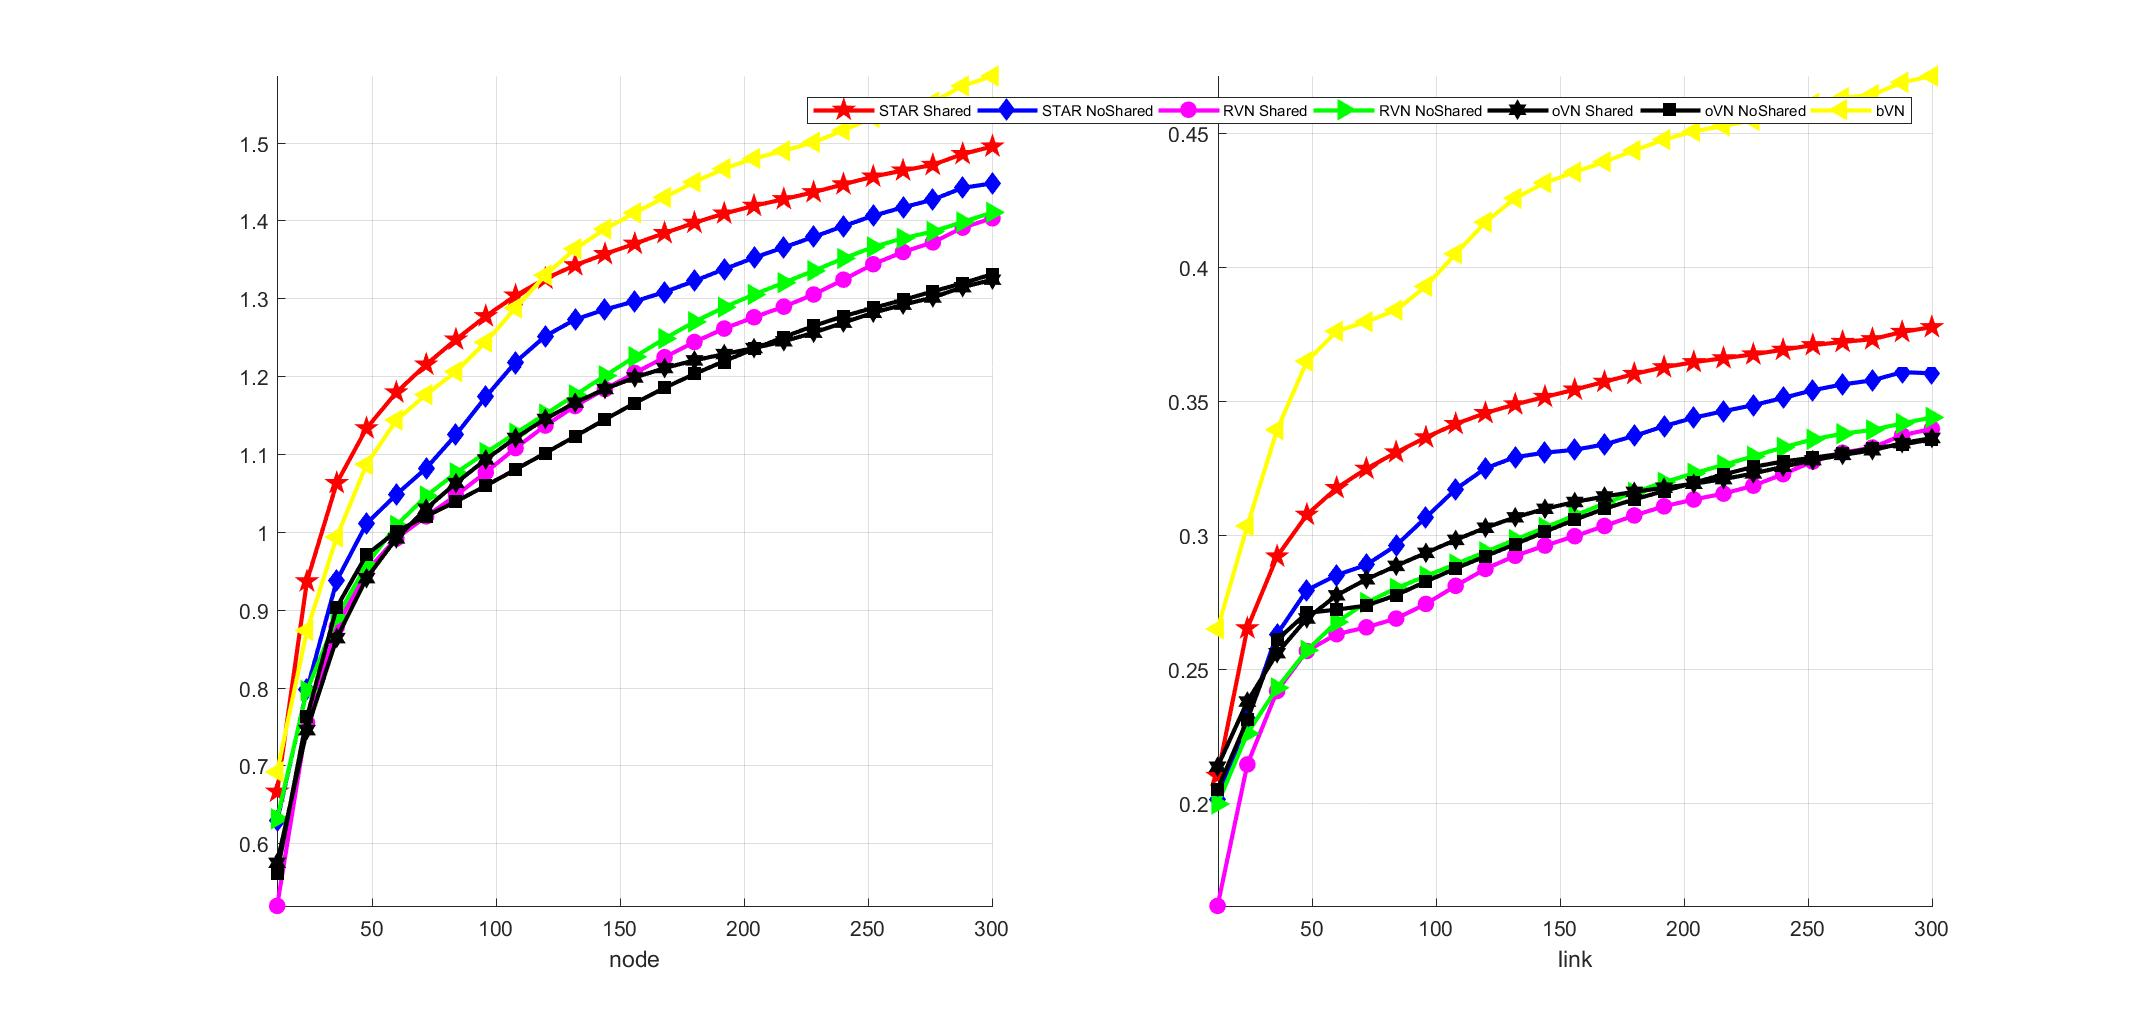
\includegraphics[width=3in]{Fig/MigrationFrequence}\\
  \caption{Migration Frequency Ratio}\label{fig:MigrationFrequence}
\end{figure}
%As mentioned above, FD-EVN algorithms achieve higher acceptance ratio and lower embedding cost at the cost of more node migration after facility node failure, which would cause service interruption and should be examined carefully, especially for the application with SLA constraints. We run our simulation in $\SubstrateNewtorkRunTimeInterval$ time unites, which corresponds to about $\SubStrateFacilityNodeFailDuration$ requests on average in each instance of simulation. The migration frequency
%after random facility node  failure is presented in Fig. 8 in terms of the number of VN nodes.


\subsection{Stress}
The stress level of a substrate entity reflects the number of virtual entities that are mapped onto it. The more virtual enti ties use the same substrate resource, the higher the impact regarding possible side effects. For example, mapping many virtual nodes onto a single substrate node keeps the CPU of the host operating system busy. A high substrate link stress might result in some additional packet delay because the resources of the substrate link and the host interfaces communicating through this link have to be shared
between virtual entities.
The stress of a SN element (node or link)is the number of virtual instances mapped on top of it.
Stress Fig.\ref{fig:Stress}:
\begin{figure}[htbp]
  \centering
  % Requires \usepackage{graphicx}
  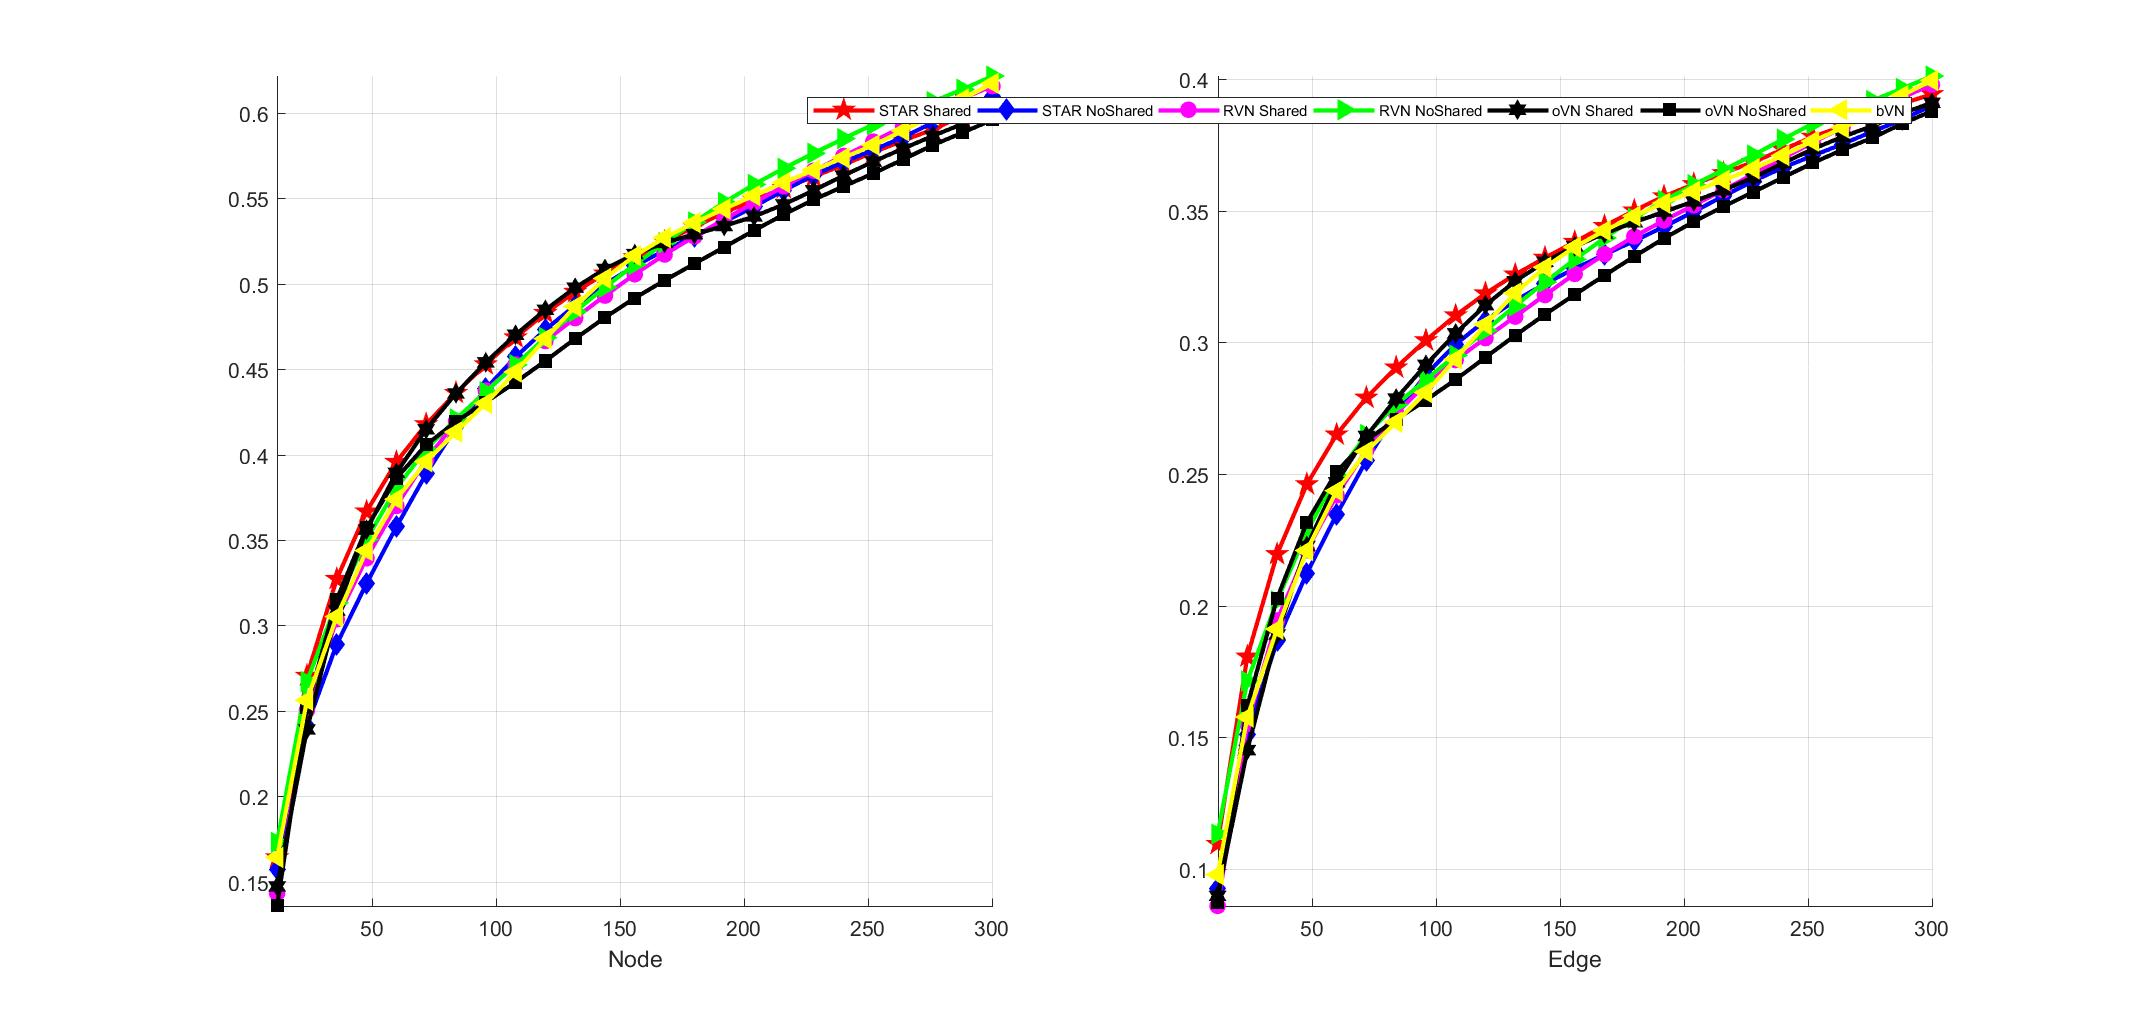
\includegraphics[width=3in]{Fig/Stress}\\
  \caption{Stress}\label{fig:Stress}
\end{figure}


\subsection{Utilization}
Utilization measures, in each SN entity (node or link), the sum of the spent substrate resources due to the mapping of virtual entities divided by the total amount of resources. This metric is a more precise measurement tool than
the stress level metric, because it also takes into account the magnitude of the resource usage instead of simply counting the number of virtual entities that use a resource. For example, to measure the utilization of a substrate node, the sum of mapped computing resources divided by the node computing capacity of the node could be used. The usage of a substrate link could be based on the sum of mapped bandwidth resources divided by the total link bandwidth capacity.

Utilization Fig.\ref{fig:Utilization}:
\begin{figure}[htbp]
  \centering
  % Requires \usepackage{graphicx}
  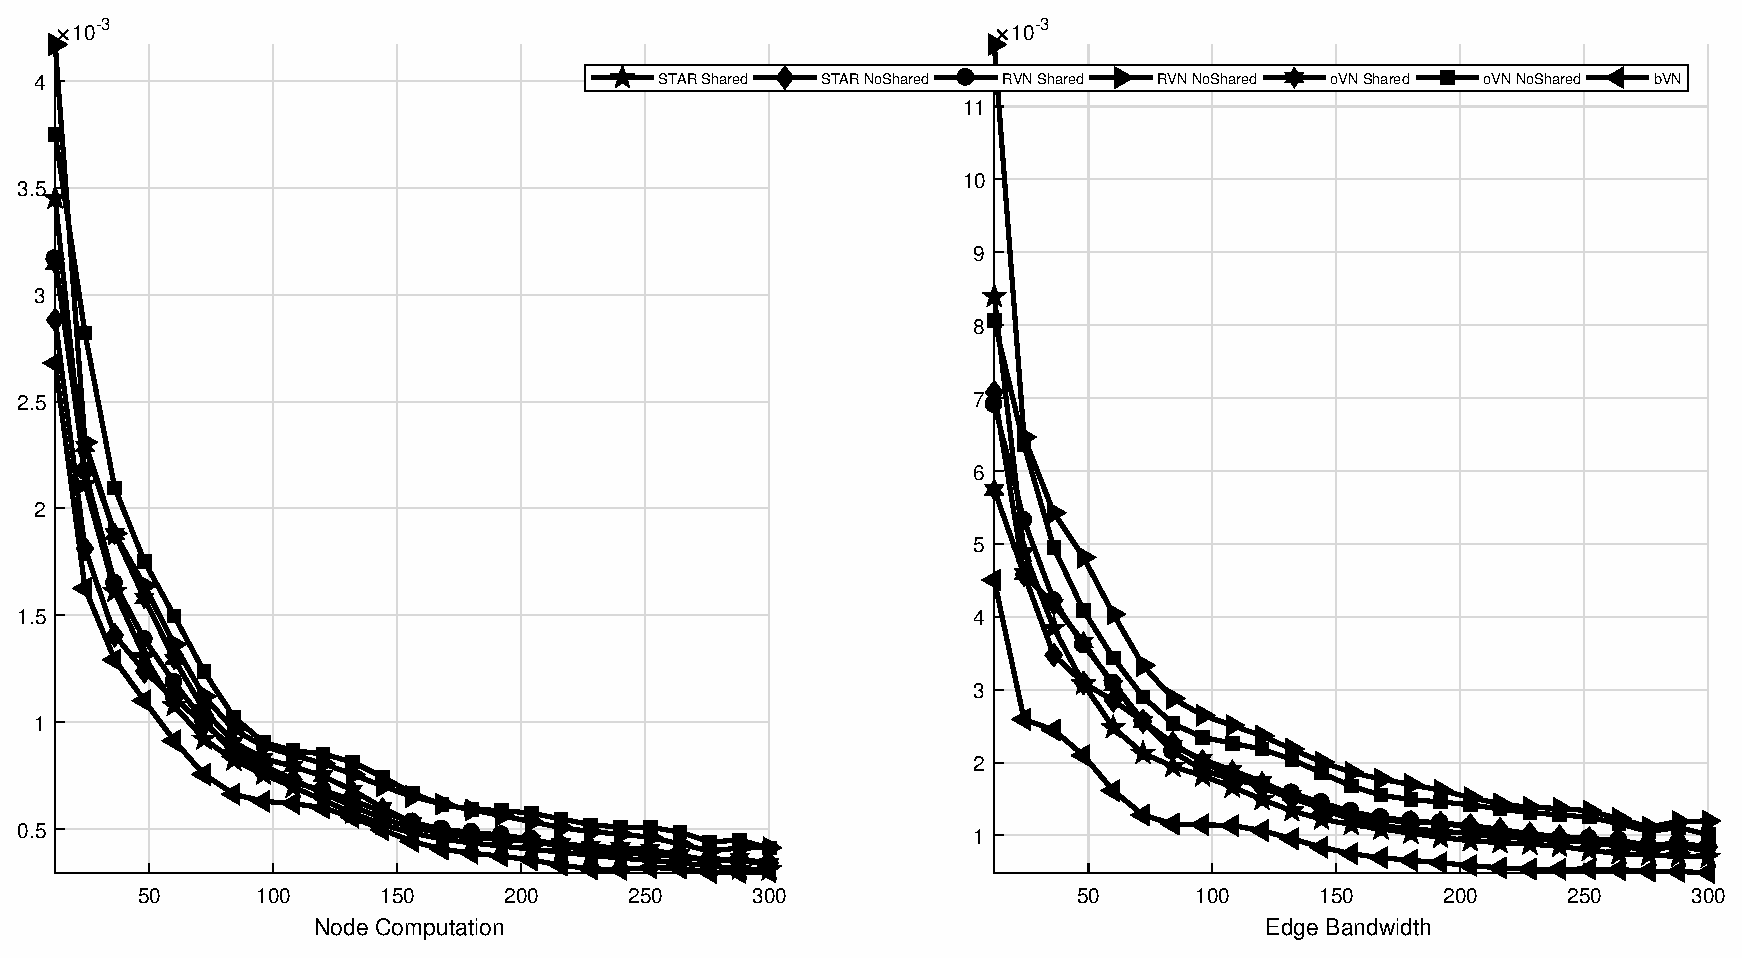
\includegraphics[width=3in]{Fig/Utilization}\\
  \caption{Utilization}\label{fig:Utilization}
\end{figure}


%\begin{figure*}
%  \centering
%  % Requires \usepackage{graphicx}
%
%
%
% \begin{equation*}
%\left[ {\begin{array}{*{20}{c}}
%&C_{P_{2.2}}&C_{P_{2.3}}&C_{P_3}&C_{P_4}&C_{B_{1.1}}&C_{B_{1.2}}&C_{B_{2.1}}&C_{B_{2.4}}&C_{B_{3.2}}&C_{B_{3.2}}\\
%{R_{V_1}}&\infty&\infty&\infty&\infty&\fbox{N+(2)+4+5+3}&\infty&${N+(2)+4+5+3}$&\infty&\infty&\infty\\
%R_{V_2}&\fbox{4}&\infty&\infty&\infty&\infty&${N+(3)+4+6}$&\infty&\infty&${N+(3)+4+6}$&\infty\\
%R_{V_3}&\infty&${M+(2)+5}$&\fbox{5}&\infty&\infty&\infty&\infty&\infty&\infty&${N+(5)+5+6}$\\
%R_{V_4}&\infty&\infty&\infty&\fbox{3}&\infty&\infty&\infty&${N+(6)+3}$&\infty&\infty\\
%\end{array}} \right]
%\end{equation*}
% \begin{equation*}
%\left[ {\begin{array}{*{20}{c}}
%&C_{P_{1}}&C_{P_3}&C_{P_4}&C_{B_{1.1}}&C_{B_{1.2}}&C_{B_{2.1}}&C_{B_{2.4}}&C_{B_{3.2}}&C_{B_{3.2}}\\
%{R_{V_1}}&4&\infty&\infty&${M+4}$&\infty&$N+(2)+4+5+3$&\infty&\infty&\infty\\
%R_{V_2}&\infty&\infty&\infty&\infty&${M+(1)+4+1} $&\infty&\infty&${N+(3)+4+6}$&\infty\\
%R_{V_3}&\infty&6&\infty&\infty&\infty&\infty&\infty&\infty&$N+(5)+5+6$\\
%R_{V_4}&\infty&\infty&0&\infty&\infty&\infty&$N+(6)+3$&\infty&\infty\\
%\end{array}} \right]
%\end{equation*}
%
% \begin{equation*}
%\left[ {\begin{array}{*{20}{c}}
%&C_{P_{1}}&C_{P_{2.2}}&C_{P_{2.3}}&C_{P_4}&C_{B_{1.1}}&C_{B_{1.2}}&C_{B_{2.1}}&C_{B_{2.4}}&C_{B_{3.2}}&C_{B_{3.3}}\\
%R_{V_1}&\fbox{5}&\infty&\infty&\infty&M+5&\infty&${N+(2)+4+5+3}$&\infty&\infty&\infty\\
%R_{V_2}&\infty&\mbox{6}&\infty&\infty&\infty&\fbox{M+6}&\infty&\infty&${N+(3)+4+6}$&\infty\\
%R_{V_3}&\infty&\infty&\fbox{M+(2)+1}&\infty&\infty&\infty&\infty&\infty&\infty&${N+(5)+5+6}$\\
%R_{V_4}&\infty&\infty&\infty&\fbox{0}&\infty&\infty&\infty&${N+(6)+3}$&\infty&\infty\\
%\end{array}} \right]
%\end{equation*}
%\end{figure*}




\subsection{Edge Weight}
Edge Weight Fig.\ref{fig:EdgeWeight}:
\begin{figure}[htbp]
  \centering
  % Requires \usepackage{graphicx}
  \includegraphics[width=3in]{Fig/EdgeWeight}\\
  \caption{EdgeWeight}\label{fig:EdgeWeight}
\end{figure}
EdgeWeightAccumulate  Fig.\ref{fig:EdgeWeightAccumulate}:
\begin{figure}[htbp]
  \centering
  % Requires \usepackage{graphicx}
  \includegraphics[width=3in]{Fig/EdgeWeightAccumulate}\\
  \caption{EdgeWeightAccumulate}\label{fig:EdgeWeightAccumulate}
\end{figure}

EdgeWeightCurrentAverage Fig.\ref{fig:EdgeWeightCurrentAverage}:
\begin{figure}[htbp]
  \centering
  % Requires \usepackage{graphicx}
  \includegraphics[width=3in]{Fig/EdgeWeightCurrentAverage}\\
  \caption{EdgeWeightCurrentAverage}\label{fig:EdgeWeightCurrentAverage}
\end{figure}

EdgeWeightAccumulateAverage Fig.\ref{fig:EdgeWeightAccumulateAverage}:
\begin{figure}[htbp]
  \centering
  % Requires \usepackage{graphicx}
  \includegraphics[width=3in]{Fig/EdgeWeightAccumulateAverage}\\
  \caption{EdgeWeightAccumulateAverage}\label{fig:EdgeWeightAccumulateAverage}
\end{figure}


\subsection{Acception Ratio with different Exponential Mean}
\begin{figure}[htbp]
  \centering
  % Requires \usepackage{graphicx}
  \includegraphics[width=3in]{Fig/AcceptionRatioExponentialMean}\\
  \caption{Acception Ratio with different Exponential Mean}\label{fig:AcceptionRatioExponentialMean}
\end{figure}

\subsection{Acception Ratio with different Possion Mean}
\begin{figure}[htbp]
  \centering
  % Requires \usepackage{graphicx}
  \includegraphics[width=3in]{Fig/AcceptionRatioPossionMean}\\
  \caption{Acception Ratio with different Possion Mean}\label{fig:AcceptionRatioPossionMean}
\end{figure}

\subsection{Node Failure}
\begin{figure}[htbp]
  \centering
  % Requires \usepackage{graphicx}
  \includegraphics[width=3in]{Fig/NodeFailure}\\
  \caption{Node Failure}\label{fig:NodeFailure}
\end{figure}


\subsection{Node Migration}
\begin{figure}[htbp]
  \centering
  % Requires \usepackage{graphicx}
  \includegraphics[width=3in]{Fig/NodeMigration}\\
  \caption{Node Failure}\label{fig:NodeMigration}
\end{figure}




%\end{CJK*}

%\appendix
%This appendix will try to clarify themain differences between
%the considered heuristics. The network which will be used
